\documentclass[a4paper]{article}
\usepackage[utf8]{inputenc}

\usepackage{amsthm}
\usepackage{amssymb}
\usepackage{amsmath}
\usepackage{mathtools}

\usepackage[ruled,vlined]{algorithm2e}
% \usepackage{algorithm}
% \usepackage{algorithmic}
\usepackage{array}
\usepackage{listings}
\usepackage{multirow}

\usepackage[dvipsnames]{xcolor}
\usepackage[toc,page]{appendix}
\usepackage{tikz}
\usepackage{float}
\usepackage{graphicx}
\usepackage{caption}
\usepackage{subcaption}
\usepackage[colorlinks = true,
            linkcolor = blue,
            urlcolor  = blue,
            citecolor = blue,
            anchorcolor = blue]{hyperref}

\graphicspath{ {images/} }
\usepackage[a4paper,width=165mm,top=22mm,bottom=22mm]{geometry}
\setlength{\headheight}{15pt}
% \usepackage[most]{tcolorbox}

\title{Mixed Martial Arts Ontology developed in OWL and SWRL}
\author{Ali Khudiyev}
\date{November 2021}

\begin{document}
\maketitle

\section{Introduction \& Modelling}
\textbf{Mixed Martial Arts (MMA)} is a full-contact combat sport based on striking, grapling and ground fighting. \href{https://www.sportsunfold.com/top-10-best-mma-organizations-promotions}{Top MMA organizations} in the world are \textit{Ultimate Fighting Championship (UFC)}, \textit{Bellator MMA}, \textit{Absolute Championship Akhmat (ACA)} which allow mixed-gender championships by separating male and female events. Such companies gain profit by selling fights as the end-user products each of which goes through the process of organization(i.e., fighter matching, place selection, pay-per-view prices, etc.) and evaluation(i.e., fight winner/drawer, fighter scoring). As in other combat sports, there are divisions among fighters participating in MMA. These divisions are to group fighters in the same weight class to make the championships fair since extra weights can be advantage and/or disadvantage depending on various factors. For example, UFC has the following weight classes\footnote{\url{https://wayofmartialarts.com/ufc-weight-classes-divisions}}:

\begin{table}[H]
	\centering
	\begin{tabular}{c|c}
		\textbf{Weight class} & \textbf{Weight} \\
		\hline
		Heavyweight & 120.2 kg \\
		\hline
		Light heavyweight & 102.1 kg \\
		\hline
		Middleweight & 83.9 kg \\
		\hline
		Welterweight & 77.1 kg \\
		\hline
		Lightweight & 70.3 kg \\
		\hline
		Featherweight & 65.8 kg \\
		\hline
		Bantamweight & 61.2 kg \\
		\hline
		Flyweight & 56.7 kg \\
		\hline
		Strawweight & 52.5 kg
	\end{tabular}
	\caption{UFC Weight Classes}
	\label{tab:ufc_divisions}
\end{table}

Building an ontology is all about observing the relevant existing concepts and the relationships between them. For MMA ontology, there are whole bunch of concepts and relationships, however, 
I will illustrate the ones that are among the most important ones that make MMA what it is. The first concepts that come to the mind in MMA are the notion of 
\textcolor{ForestGreen}{organization} and \textcolor{ForestGreen}{person}. An MMA \textcolor{ForestGreen}{organization} \textcolor{orange}{has a name} and 
\textcolor{orange}{pays} monthly salary to the \textcolor{ForestGreen}{organization workers}. Organization workers can be \textcolor{ForestGreen}{CEO}, \textcolor{ForestGreen}{judges}, 
\textcolor{ForestGreen}{referees}, \textcolor{ForestGreen}{organizers} and \textcolor{ForestGreen}{fighters}. \textcolor{ForestGreen}{Fighters} \textcolor{orange}{participates at} 
\textcolor{ForestGreen}{fights} which is \textcolor{orange}{organized by} \textcolor{ForestGreen}{organizers}, \textcolor{orange}{controlled by} \textcolor{ForestGreen}{referees} and
\textcolor{orange}{judged by} \textcolor{ForestGreen}{judges}. \textcolor{ForestGreen}{Judges} \textcolor{orange}{gives} \textcolor{ForestGreen}{points} to both \textcolor{ForestGreen}{fighters} 
based on which it is decided which \textcolor{ForestGreen}{fighter} \textcolor{orange}{won}/\textcolor{orange}{lost}/\textcolor{orange}{drawed} the \textcolor{ForestGreen}{fight}.
The \textcolor{ForestGreen}{fight} \textcolor{orange}{takes place at} some \textcolor{ForestGreen}{location} and at a specific \textcolor{ForestGreen}{time}, \textcolor{orange}{costs} some 
amount of money which can be \textcolor{orange}{paid by} a \textcolor{ForestGreen}{non organization worker} to \textcolor{orange}{buy} the \textcolor{ForestGreen}{fight}. Every fight 
\textcolor{orange}{has a division} that restricts how much the participating \textcolor{ForestGreen}{fighters} \textcolor{orange}{weigh}. Any two \textcolor{ForestGreen}{fighters} 
have to \textcolor{orange}{have gender} that is either male or female, in other words, (male vs female) match is impossible due to unfairness. The \textcolor{ForestGreen}{organization} 
have certain age restrictions for its \textcolor{ForestGreen}{workers} and also \textcolor{orange}{pays bonus} money to a winning \textcolor{ForestGreen}{fighter}.
In this briefly written text, green words refer to concepts and orange ones refer to relations between them. Notion of classes, object and data properties become obvious by just reading this paragraph. 
The whole information described here can be represented as the knowledge graph shown below.

\begin{figure}[H]
	\centering
	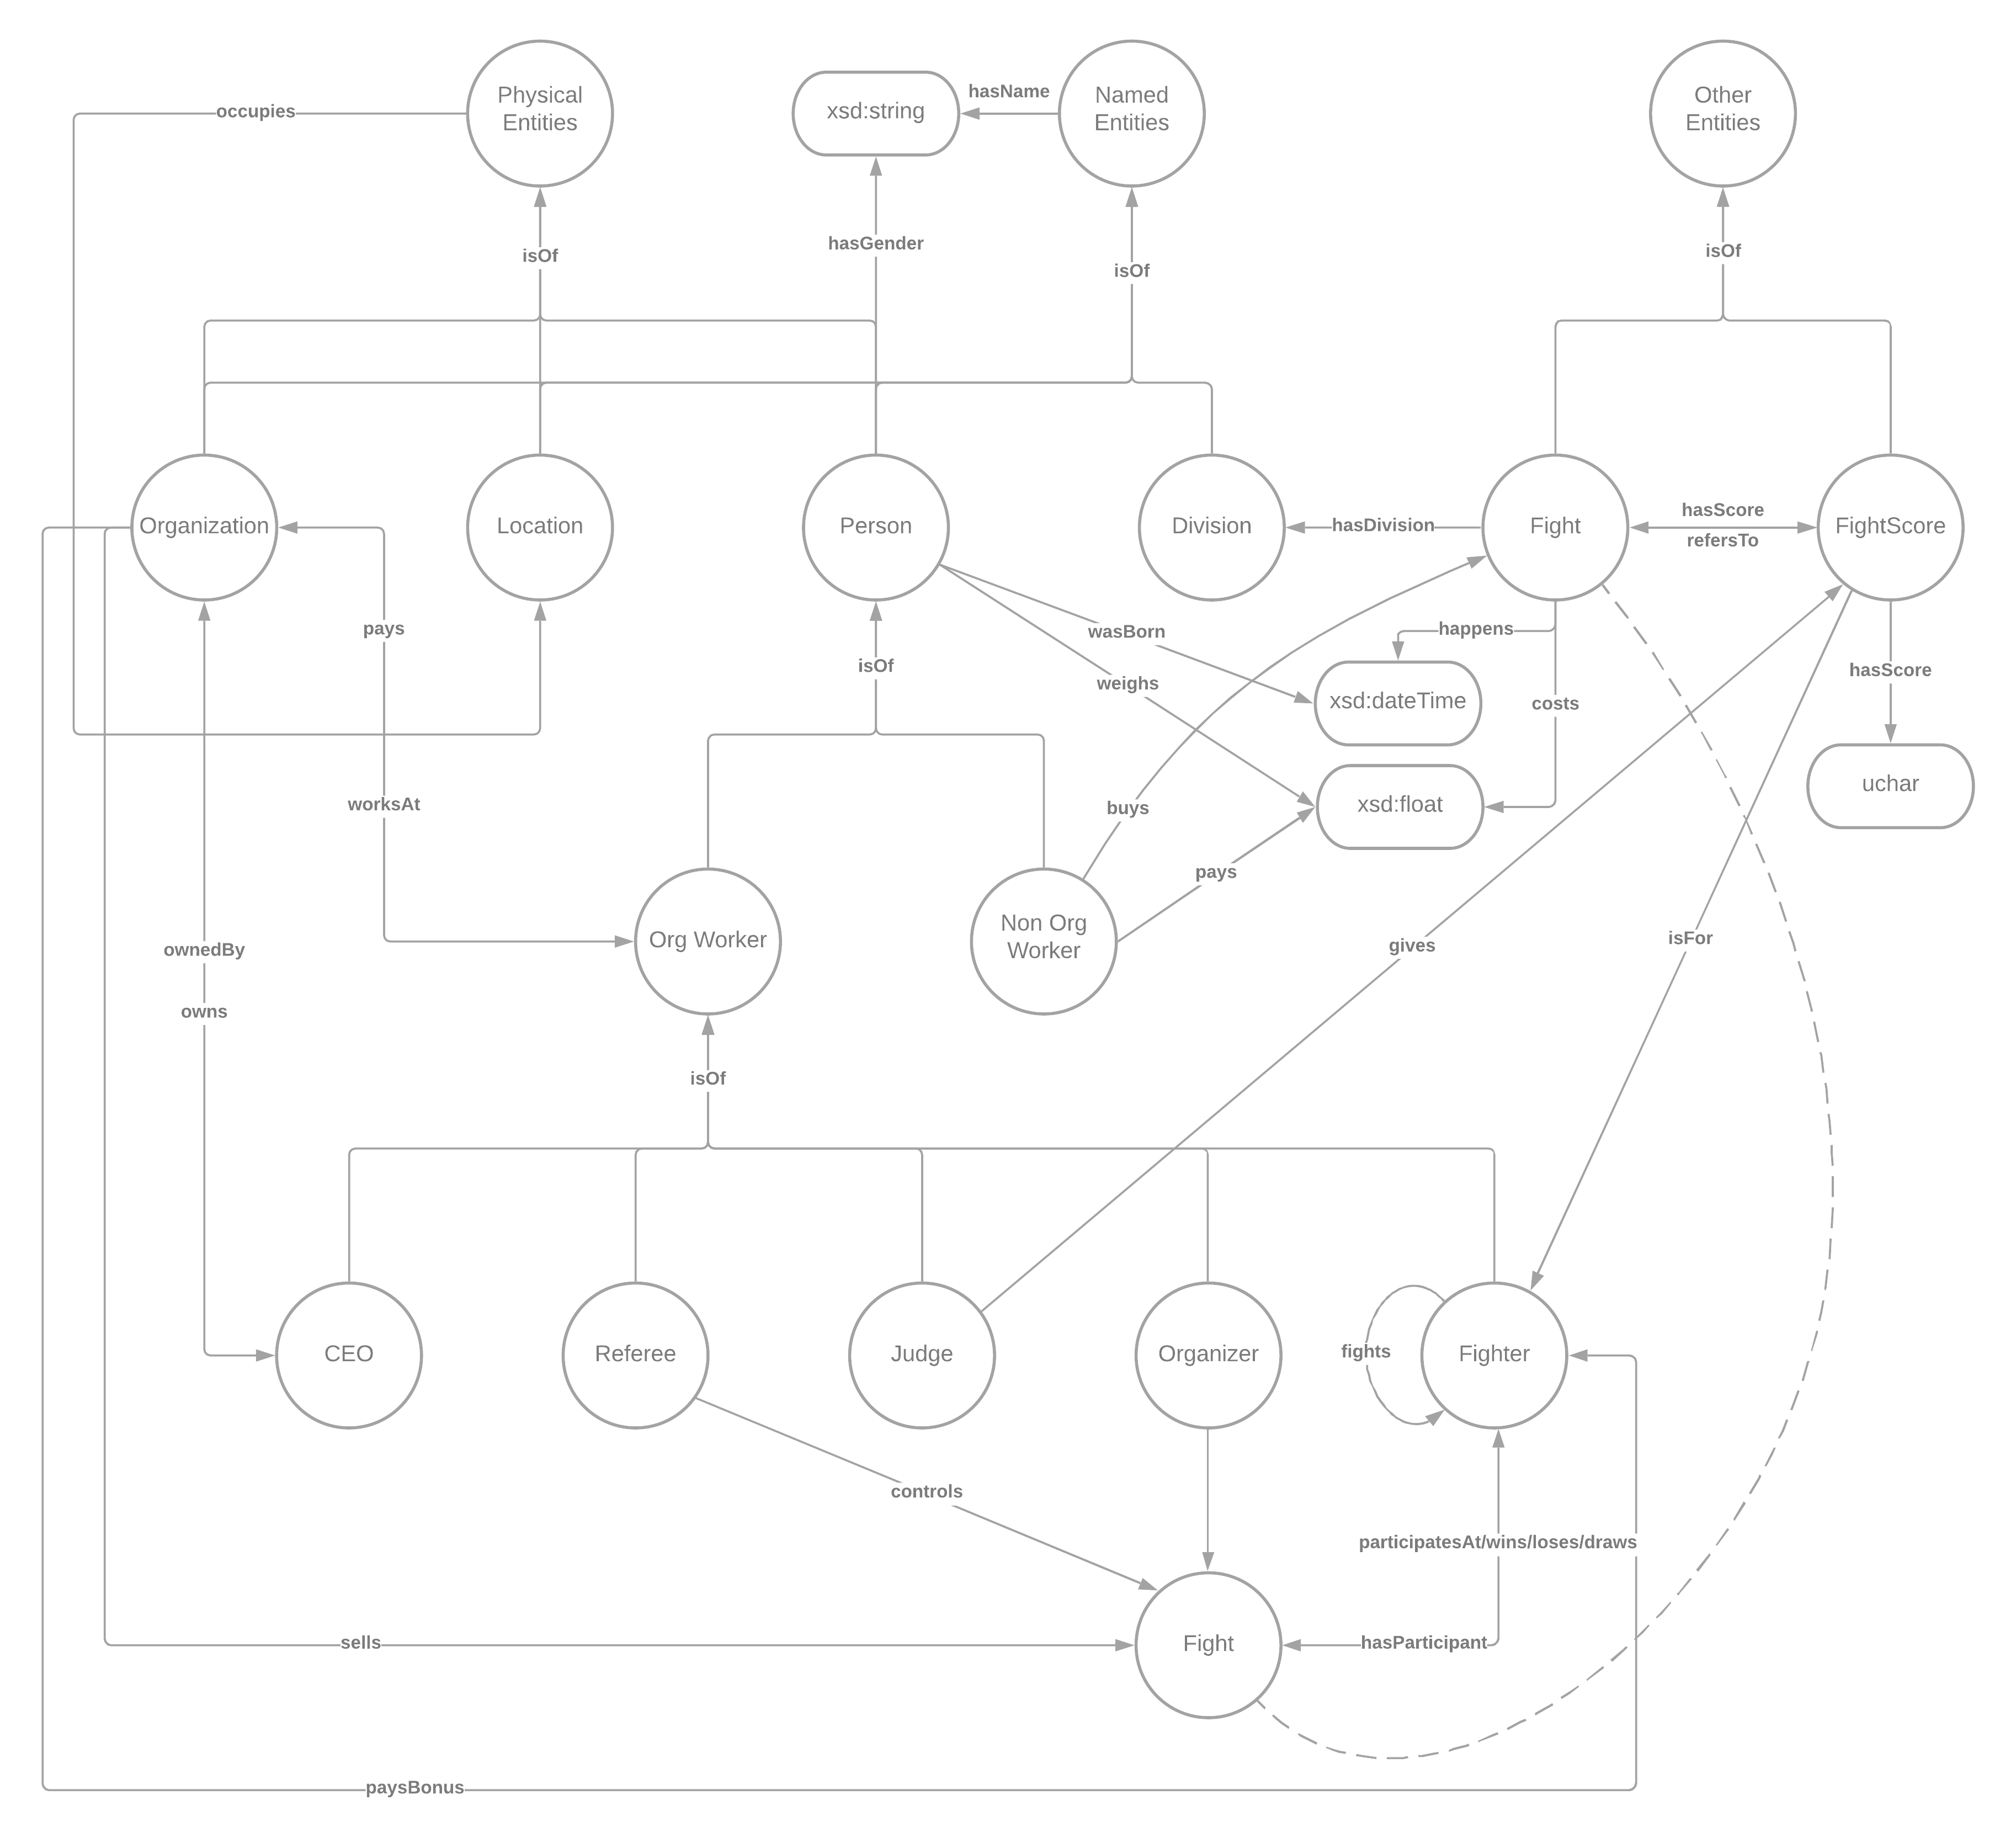
\includegraphics[width=0.75\textwidth]{resources/mma_onto.png}
	\caption{MMA Ontology Graph}
	\label{fig:mma_ontology}
\end{figure}

In figure \ref{fig:mma_ontology}(see appendix \ref{appendix:ontograf_graph} for the complete graph generated by \textit{Ontograf} plugin), arrows represent relations or properties, 
circles represent objects and rectangles represent data types. The properties that link 2 objects are called object properties whereas the ones that link an object with a data type 
are called data properties. However, it is not enough to represent the whole just by using OWL alone and in fact, there are complementary axioms which represent some of the relationships 
hidden in the OWL graph. There are several rules that are among the most relevant ones as far as this project concerns and they are shown below in DL.

\begin{equation}
	\text{Fight} \sqsubseteq =2\text{hasParticipant}.\text{Fighter} \sqcap =1\text{hasDivision}.\text{Division}
	\label{formula:axiom_fight}
\end{equation}

\begin{equation}
	\text{Person} \equiv \text{OrgWorker} \sqcup \text{NonOrgWorker}
	\label{formula:axiom_person}
\end{equation}

\begin{equation}
	\text{OrgWorker} \equiv \text{Person} \sqcap \exists \text{worksAt}.\text{Organization}
	\label{formula:axiom_orgworker}
\end{equation}

\begin{equation}
	\text{CEO} \equiv \text{OrgWorker} \sqcap \exists \text{owns}.\text{Organization}
	\label{formula:axiom_ceo}
\end{equation}

\begin{equation}
	\text{Fighter} \equiv \text{OrgWorker} \sqcap \exists \text{participatesAt}.\text{Fight}
	\label{formula:axiom_fighter}
\end{equation}

\begin{equation}
	\text{Division} \equiv \text{NamedEntities} \sqcap \{D1, D2, \dots, D9\}
	\label{formula:axiom_division}
\end{equation}

\begin{equation}
	\text{Referee} \sqsubseteq \exists \text{controls}.\text{Fight}
	\label{formula:axiom_referee}
\end{equation}

\begin{equation}
	\text{Judge} \sqsubseteq \exists \text{gives}.\text{FightScore}
	\label{formula:axiom_judge}
\end{equation}

\begin{equation}
	\text{Organizer} \sqsubseteq \exists \text{organizes}.\text{Fight}
	\label{formula:axiom_organizer}
\end{equation}

Axiom (\ref{formula:axiom_fight}) indicates that any fight has to have exactly 2 participating fighters and a single division, however, the concept of fight is not strictly defined by the number of participants.
The axioms (\ref{formula:axiom_person}-\ref{formula:axiom_division}) are to define equivalence between concepts that have strict definitions in this ontology. For example, the second axiom 
states that any person is either an organization worker or a non organization worker which is inherently true, and the sixth one is to define the concept of division(weight class) as one of 9 
divisions(i.e., heavyweight, light heavyweight, lightweight and so on). The axioms from \ref{formula:axiom_referee} to \ref{formula:axiom_organizer} show relationship between referees/judges/organizers 
and people who control/give/organize some fight/fightscore/fight with the minimum cardinality of 1.

\begin{align}
	\text{Organizer}(?o) \land \text{Fight}(?f) \land \text{sells}(?o, ?f) \land \text{wins}(?x, ?f) \rightarrow paysBonus(?o, ?x)
	\label{formula:swrl_bonusRule}
\end{align}

\begin{align}
	\text{Fight}(?f) \land \text{hasDivision}(?f, D1) \land \text{hasParticipant}(?f, ?x) &\rightarrow \text{weighs}(?x, 52.5) \\
	\text{Fight}(?f) \land \text{hasDivision}(?f, D2) \land \text{hasParticipant}(?f, ?x) &\rightarrow \text{weighs}(?x, 56.7) \\
	\dots &\rightarrow \dots \\
	\text{Fight}(?f) \land \text{hasDivision}(?f, D9) \land \text{hasParticipant}(?f, ?x) &\rightarrow \text{weighs}(?x, 120.2) \\
	\label{formula:swrl_weightClasses}
\end{align}

\begin{equation}
	\begin{split}
		\text{Organizer}(?o) &\land \text{Fight}(?f) \land \text{sells}(?o, ?f) \land \text{hasParticipant}(?f, ?x) \land \\ 
							&\land \text{hasParticipant}(?f, ?y) \land \text{differentFrom}(?x, ?y) \land \\ 
							&\land \text{hasGender}(?x, ?g) \rightarrow \text{hasGender}(?y, ?g)
	\end{split}
	\label{formula:swrl_genderRule}
\end{equation}

\begin{equation}
	\begin{split}
		\text{isFor}(?fs1, ?x) &\land \text{isFor}(?fs2, ?y) \land \text{differentFrom}(?x, ?y) \land \text{refersTo}(?fs1, ?f) \land \\
							&\land \text{refersTo}(?fs2, ?f) \land \text{hasScore}(?fs1, ?s1) \land \text{hasScore}(?fs2, ?s2) \land \\ 
							&\land swrlb:equal(?s1, ?s2) \rightarrow \text{draws}(?x, ?f) \land \text{draws}(?y, ?f)
	\end{split}
	\label{formula:swrl_drawers}
\end{equation}

\begin{equation}
	\begin{split}
		\text{isFor}(?fs1, ?x) &\land \text{isFor}(?fs2, ?y) \land \text{differentFrom}(?x, ?y) \land \text{refersTo}(?fs1, ?f) \land \\
							&\land \text{refersTo}(?fs2, ?f) \land \text{hasScore}(?fs1, ?s1) \land \text{hasScore}(?fs2, ?s2) \land \\ 
							&\land swrlb:greaterThan(?s1, ?s2) \rightarrow \text{wins}(?x, ?f) \land \text{loses}(?y, ?f)
	\end{split}
	\label{formula:swrl_winner_loser}
\end{equation}

\begin{equation}
		\text{refersTo}(?fs1, ?f) \land \text{refersTo}(?fs2, ?f) \land \text{gives}(?j, ?fs1) \rightarrow \text{gives}(?j, ?fs2)
	\label{formula:swrl_judge_score}
\end{equation}

The SWRL rule \ref{formula:swrl_bonusRule} states that any fighter with the minimum record of 1 won fight is paid bonus money by the organization, rules for weight classes(till 
\ref{formula:swrl_weightClasses}) asserts fighters' weights fighting in a certain division. The rule \ref{formula:swrl_genderRule} indicates that the fighters with different genders 
cannot fight against each other and likewise, it is true for the weight classes. To be able to obtain winners/losers/drawers, rules \ref{formula:swrl_winner_loser}-\ref{formula:swrl_drawers} 
compare the scores of both fighters and conclude one of three possibilites: winner/loser, loser/winner and drawer/drawer with regard to both fighters. The last rule indicates that a judge 
who gives a score to a fighter for particular fight is also the one who gives a score to the other fighter for the same fight. There are a few more rules that are discussed later on with 
implementation details in Prot\'eg\'e.

\section{Implementation in Prot\'eg\'e}
The implementation goes through several stages: \textit{creating class hierarchy and defining class equivalance(s)/ subsumption(s)/ disjuntion(s)}, then \textit{defining relations}, 
\textit{defining SWRL rules} and finally \textit{creating individuals} to test and observe the implications. The class hierarchy is created by simply creating concepts used in the 
ontology and the class properties such as equivalance\footnote{Although equivalance is rarely used as it is mainly for merging two separately developed ontologies, there are classes 
which make it relevant to use it in this project.}, subsumption, disjuction between them are defined within the scope of the same classes. Relations are to link different concepts 
with their relevant predicates and have properties(i.e., reflexivity, transivity, etc.) as well. These 2 steps are what can be done using only OWL and they are carefully developed 
to avoid unintentional situations later on. The third step, which is defining SWRL rules, is developed by using SWRLTab in Prot\'eg\'e and tested with the OWL individuals that are 
created at the final development step of the ontology.

\subsection{Creating and Defining Classes}
Concepts or classes used in this ontology have been shown with UML class diagram in the previous modelling section. The diagram also covers object and data properties for all classes and it 
can be observed that there are several concepts that share the same properties. For example, \textit{organization}, \textit{person} and \textit{location} are concepts that have names and 
occupy some place on the Earth described by the couple of properties \textit{hasName} and \textit{occupies} respectively. In addition to these 3 classes, the \textit{division} has also a name 
but it does not occupy any place since it is an intangible object. Due to such similarities and/or dissimilarities between such concepts, 3 top-level concepts have been implemented to encapsulate 
the relavant or similar subclasses. These top-level classes are \textit{NamedEntities}, \textit{PhysicalEntities} and \textit{OtherEntities} and the rest are defined as shown below.

\begin{figure}[H]
\centering
\begin{subfigure}{.3\textwidth}
	\centering
	\begin{itemize}
		\item NamedEntities
		\begin{itemize}
			\item Organization
			\item Location
			\item Division
			\item Person
			\begin{itemize}
				\item NonOrgWorker
				\item OrgWorker
				\begin{itemize}
					\item CEO
					\item Judge
					\item Referee
					\item Organizer
					\item Fighter
				\end{itemize}
			\end{itemize}
		\end{itemize}
	\end{itemize}
	% \caption{A subfigure}
	\label{fig:name_entities}
\end{subfigure}%
\begin{subfigure}{.3\textwidth}
	\centering
	\begin{itemize}
		\item PhysicalEntities
		\begin{itemize}
			\item Organization
			\item Location
			\item Person
			\begin{itemize}
				\item NonOrgWorker
				\item OrgWorker
				\begin{itemize}
					\item CEO
					\item Judge
					\item Referee
					\item Organizer
					\item Fighter
				\end{itemize}
			\end{itemize}
		\end{itemize}
	\end{itemize}
	\vspace{1.5em}
	% \caption{A subfigure}
	\label{fig:physical_entities}
\end{subfigure}%
\begin{subfigure}{.3\textwidth}
	\centering
	\begin{itemize}
		\item OtherEntities
		\begin{itemize}
			\item Fight
			\item FightScore
		\end{itemize}
	\end{itemize}
	\vspace{13em}
	% \caption{A subfigure}
	\label{fig:other_entities}
\end{subfigure}
\caption{owl:Thing subclasses}
\label{fig:top_classes}
\end{figure}

It is more relevant to have a class hierarchy as shown in figure \ref{fig:top_classes} since it is obvious that the domain of \textit{hasName} object property is just \textit{NamedEntities} 
and the domain of \textit{occupies} object property is \textit{PhysicalEntities} class where as elements of \textit{OtherEntities} can neither have names nor occupy locations.

\subsubsection{Disjoint classes}
Disjoint classes are useful when we semantically separate distinct sets whose elements are guaranteed to be different from each other. The benefits of doing so is to be able to increase accuracy 
and sufficency of inference made with non-unique name assumption. List of the disjoing classes in this ontology is shown below.

\begin{table}[H]
	\centering
	\begin{tabular}{c|c}
		\hline
		\textbf{Class} & \textbf{Disjoint with} \\
		\hline
		OtherEntities & NamedEntities, PhysicalEntities \\
		NamedEntities & OtherEntities \\
		PhysicalEntities & OtherEntities \\
		\hline
		NonOrgWorker & OrgWorker \\
		OrgWorker & NonOrgWorker \\
		\hline
		CEO & Fighter, Referee, Judge, Organizer \\
		Fighter & CEO, Referee, Judge, Organizer \\
		Referee & CEO, Fighter, Judge, Organizer \\
		Judge & CEO, Fighter, Referee, Organizer \\
		Organizer & CEO, Fighter, Referee, Judge \\
		\hline
	\end{tabular}
	\caption{Disjoint classes in Prot\'eg\'e}
	\label{tab:disjoint_classes}
\end{table}
Equivalence of classes is not commonly used while developing an ontology since it is often useful for merging separately developed ontologies. However, it is useful for this particular ontology when we 
talk about the classes \textit{Person}, \textit{OrgWorker}, \textit{CEO}, \textit{Fighter} and \textit{Division}. In Prot\'eg\'e, equivalence relations are defined by using \underline{Equivalent To} 
description. Here are the equivalence relations rewritten in Prot\'eg\'e:

\begin{table}[H]
	\centering
	\begin{tabular}{c|c}
		\hline
		\textbf{Class} & \textbf{Equivalent To} \\
		\hline
		Person & OrgWorker \textcolor{cyan}{or} NonOrgWorker \\
		\hline
		OrgWorker & Person \textcolor{cyan}{and} (worksAt \textcolor{cyan}{some} Organization) \\
		\hline
		CEO & OrgWorker \textcolor{cyan}{and} (owns \textcolor{cyan}{some} Organization) \\
		\hline
		Fighter & OrgWorker \textcolor{cyan}{and} (participatesAt \textcolor{cyan}{some} Fight) \\
		\hline
		Division & NamedEntities \textcolor{cyan}{and} \{D1, D2, \dots, D9\} \\
	\end{tabular}
	\caption{Equivalence in Prot\'eg\'e}
	\label{tab:protege_equivalence}
\end{table}

\subsubsection{Classes under subclass-of}
From the hierarchy of classes shown previosly, subclass-of relations between classes are already obvious. In addition to obvious ones, the implementation is a bit more detailed; there are some classes 
that are not simply a subclass of another user-defined class but also \textit{dynamically created classes}\footnote{Class all of whose elements satisfy the given set of formulas.} by Prot\'eg\'e. 
For example, \textit{Fight} is of \textit{OtherEntities} and subclass of a class each of whose elements has 2 different participating fighters. To add a new subclass-of relation in Prot\'eg\'e, 
\underline{SubClass Of} description is used.

\begin{table}[H]
	\centering
	\begin{tabular}{c|c}
		\hline
		\textbf{Class} & \textbf{SubClass Of} \\
		\hline
		 		& OtherEntities \\
		Fight	& hasParticipant \textcolor{cyan}{exactly} 2 Fighter \\
				& hasDivision \textcolor{cyan}{exactly} 1 Division \\
		\hline
					& OtherEntities \\
		FightScore	& isFor \textcolor{cyan}{exactly} 2 Fighter \\
					& refersTo \textcolor{cyan}{exactly} 1 Fight \\
		\hline
		Person & NamedEntities \textcolor{cyan}{and} PhysicalEntities \\
		\hline
		Judge & OrgWorker \textcolor{cyan}{and} (gives \textcolor{cyan}{gives} FightScore) \\
		\hline
		Referee & OrgWorker \textcolor{cyan}{and} (controls \textcolor{cyan}{some} Fight) \\
		\hline
		Organizer & OrgWorker \textcolor{cyan}{and} (organizes \textcolor{cyan}{some} Fight) \\
		\hline
		Organization & NamedEntities \textcolor{cyan}{and} PhysicalEntities \\
		\hline
		Location & NamedEntities \textcolor{cyan}{and} PhysicalEntities \\
	\end{tabular}
	\caption{Subclass-of in Prot\'eg\'e}
	\label{tab:protege_subclassof}
\end{table}

\subsection{Defining Relations}
A relation in logic has some arity, which is usually called k-ary relation. When $k$ is 1, it is called unary and when $k$ is 2, it is called binary relation. In Prot\'eg\'e, only binary relations are 
developed and therefore, we give off some level of expressiviness as a trade-off with reduced computation complexity. Due to such expressivity, any relation with more than arity 2 has to be reformulated with the 
help of additional concepts and relations. It is the same case with the classes \textit{Fight}, \textit{FightScore} and \textit{Fighter} in this project; as it is impossible to have a 3-ary relation 
describing a \textit{score} of \textit{fighter} in a particular \textit{fight}. There are also several properties of binary relations such as functional, symmetric, reflexive, transtive and so on 
that describes the nature of the relation. These properties are also used in the developement when it is relevant and necessary to avoid illogical KB(Knowledge Base) and/or inferences.

\begin{table}[H]
	\centering
	\begin{tabular}{|m{0.15\textwidth}|m{0.17\textwidth}|m{0.17\textwidth}|m{0.17\textwidth}|m{0.2\textwidth}|}
		\hline
		\textbf{Relation} & \textbf{Domain} & \textbf{Range} & \textbf{Type} & \textbf{Description} \\
		\hline
		costs & Fight & xsd:float & functional & Fight costs some amount of money \\
		\hline
		happens & Fight & xsd:dateTime & functional & Fight happens at some date \\
		\hline
		hasGender & Person & xsd:string & functional & Person has a gender \\
		\hline
		hasName & NamedEntities & xsd:string & functional & Any concept has a name \\
		\hline
		hasScore & FightScore & xsd:unsignedByte & functional & Fight score is an 8 bit positive integer \\
		\hline
		pays & NonOrgWorker & xsd:float & - & Non organization worker pays some amount of money to buy fights \\
		\hline
		wasBorn & Person & xsd:dateTime & functional & Person was born at some date time \\
		\hline
		weighs & Person & xsd:float & functional & Person has a weight \\
		\hline
	\end{tabular}
	\caption{Data properties}
	\label{tab:data_props}
\end{table}

The MMA ontology does not concern about changing facts through time and therefore, it can contain functional relations such as \textit{weighs} that represent state of an object at a particular slice of time. 
In addition to data properties shown in the table \ref{tab:data_props}, all object properties are listed in the table \ref{tab:object_props}(see appendix \ref{appendix:object_props}).

\subsection{Defining SWRL Rules}
SWRL rules can be defined in Prot\'eg\'e by accessing \textit{SWRLTab} plugin since the software does not inherently support such rules. The rules have to be in horn clauses, in other words, 
only one positive literal is allowed in the formula. Here are the complete list of rules created in Prot\'eg\'e:

\begin{figure}[H]
	\centering
	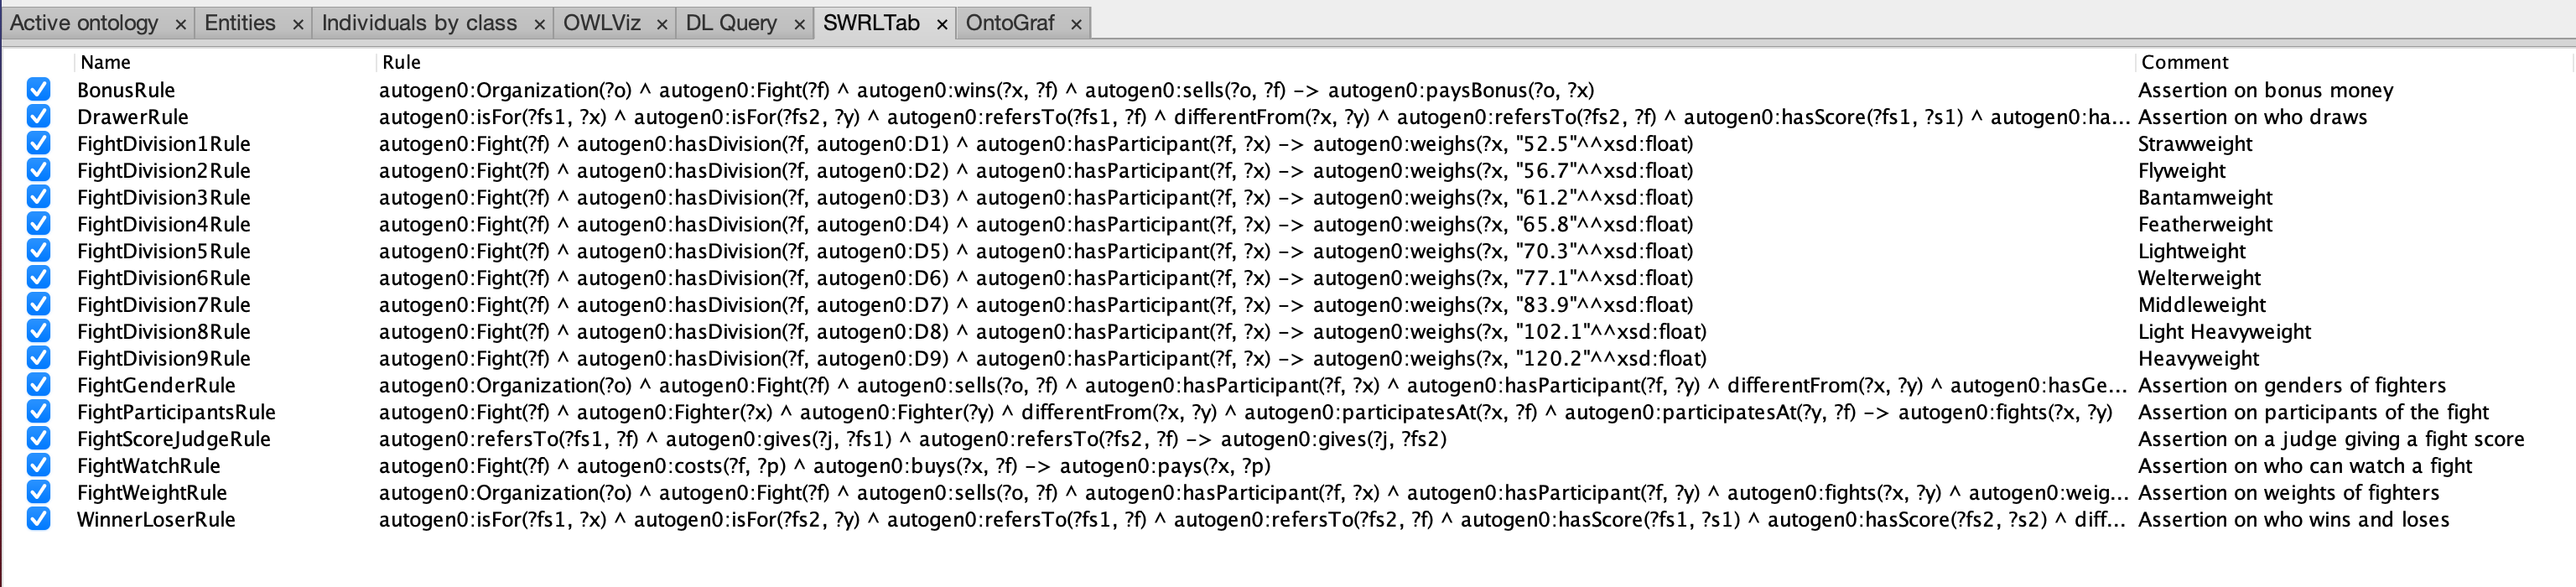
\includegraphics[width=0.8\textwidth]{resources/swrl_rules.png}
	\caption{SWRL rules implemented in Prot\'eg\'e}
	\label{fig:swrl_rules_protege}
\end{figure}

There are extra implemented rules shown in the figure \ref{fig:swrl_rules_protege} which are also helpful for certain situations. For example, the rule \textit{FightWeightRule} asserts that any 
couple of fighters, who fight against each other, have to be in the same weight class and \textit{FightParticipantsRule} reads that 2 fighters fight against each other if they are participants 
of the same fight. In the other hand, the rule \textit{FightWatchRule} is used to derive the fact that any non-organization worker, who has bought the fight, has also paid money for it.

\subsection{List of Individuals}
There are a bunch of individuals in the ontology, however, a few are discussed in this paper. The important individuals that are shown below(table \ref{tab:asserted}) are the ones for which 
reasoner inferred more/interesting information than others. The list of some created individuals and inferences on them are given in the table \ref{tab:all_individuals}(see appendix \ref{appendix:individuals}).

\begin{table}[H]
	\centering
	\begin{tabular}{|c|c|}
		\hline
		\textbf{Individual} & \textbf{Asserted} \\
		\hline
		Org & Organization \\
			& sells Fight1, sells Fight2 \\
			& hasName UFCA \\
		\hline
		OrgCEO & Person \\
			& owns Org \\
			& hasName Nihad \\
		\hline
		OrgCEO2 & owns Org \\
		\hline
		OrgFighter1 & participatesAt Fight1 \\
			& hasGender male \\
			& hasName Telman \\
		\hline
		OrgFighter2 & Fighter \\
			& hasName Bashir \\
		\hline
		Fight1 & hasDivision D1 \\
			& hasGivenScore FightScore1\_2 \\
			& hasParticipant OrgFighter2, costs 25.0 \\
		\hline
		FightScore1\_1 & FightScore \\
			& isFor OrgFighter1 \\
			& refersTo Fight1, hasScore 15 \\
		\hline
		FightScore1\_2 & FighScore \\
			& isFor OrgFighter2, hasScore 17 \\
		\hline
	\end{tabular}
	\caption{Individuals}
	\label{tab:asserted}
\end{table}

% bonus section
\subsection{SPARQL Queries}
SPARQL helps to send queries to the knowledge base and it is not supposed to work with the inferred data unlike Snap SPARQL. A simple query is shown in the figure below which essentially asks for the 
data that matches the given conditions. In this example, the query reads that any individual(fighter) who has a specified gender, name and a given score according to the fights fought. Only single 
fighter was returned since \textit{OrgFighter1} is the only one that has an explicitly specified gender and \textit{participates at} some fight(\textit{Fight1}).

\begin{figure}[H]
	\centering
	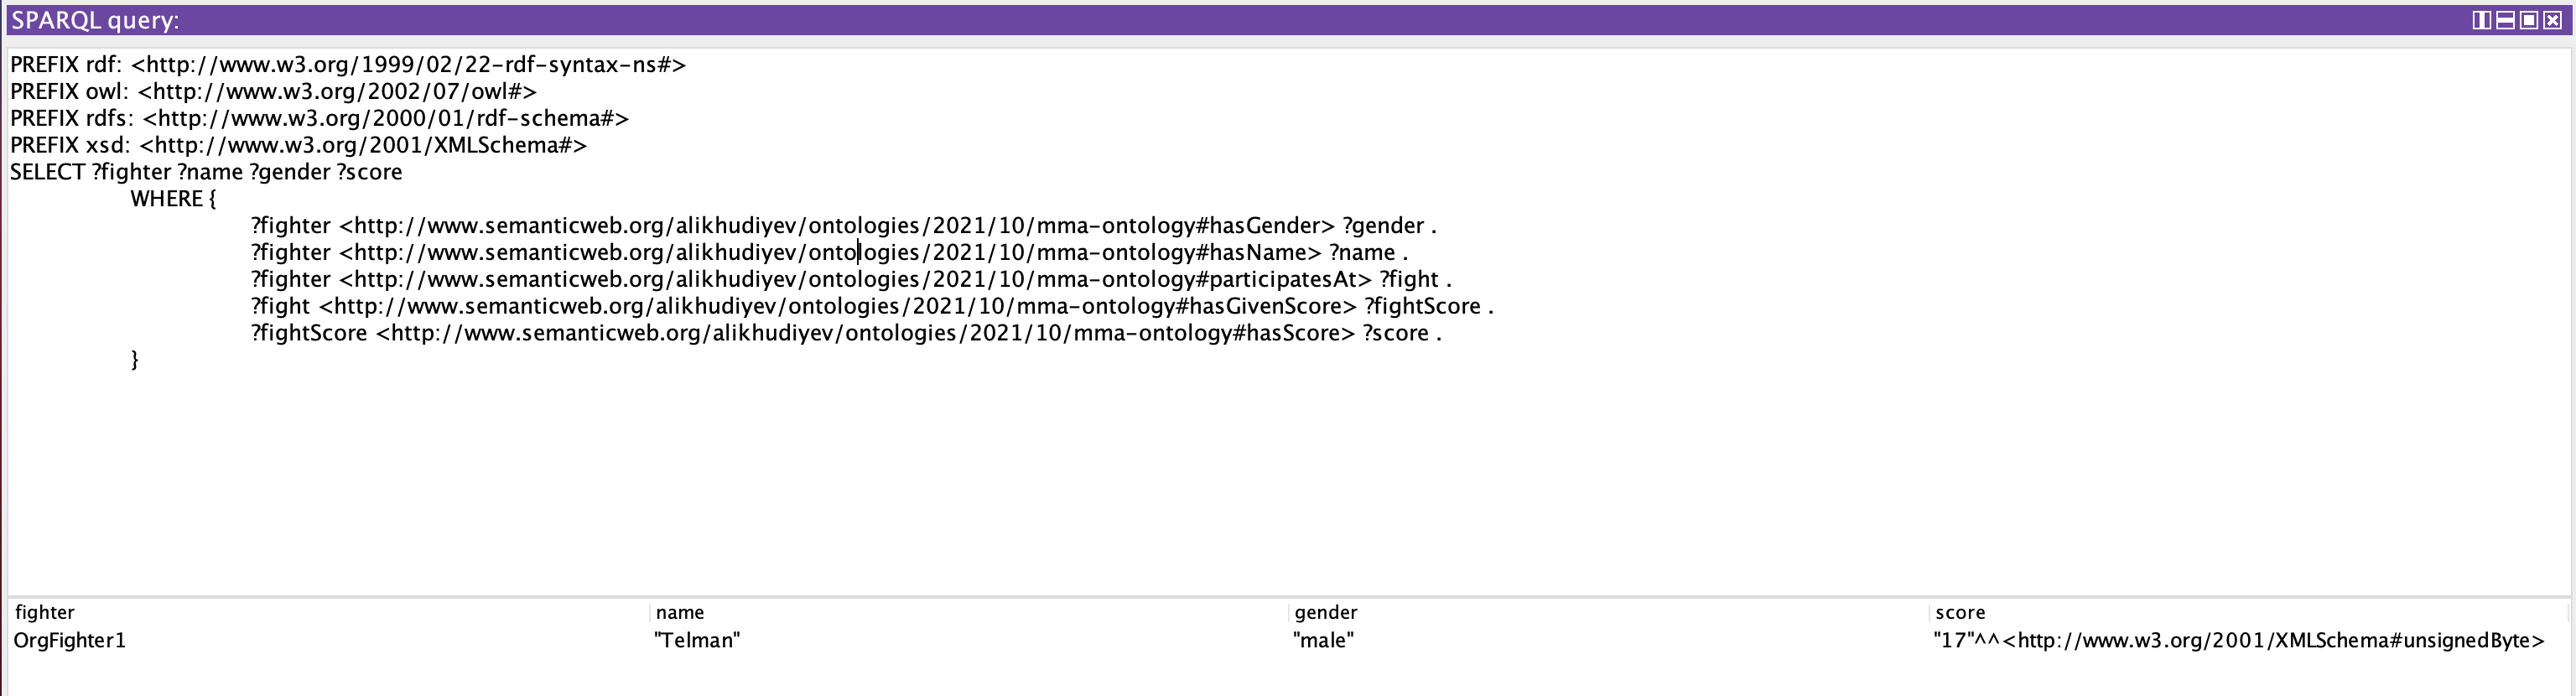
\includegraphics[width=0.8\textwidth]{resources/sparql1.png}
	\caption{Simple Query}
	\label{fig:sparql1}
\end{figure}

The SPARQL query shown below uses \underline{UNION} and \underline{FILTER} keywords that helps to group and filter individuals respectively. First, all individuals named \textit{UFCA}(Org), 
\textit{Nihad}(OrgCEO), \textit{Narmin}(OrgFighter4) and \textit{Gulshan}(-) are grouped together and then filtered according to their specified genders. In this example, all males are filtered while 
females or any individuals with any unspecified gender are dropped.

\begin{figure}[H]
	\centering
	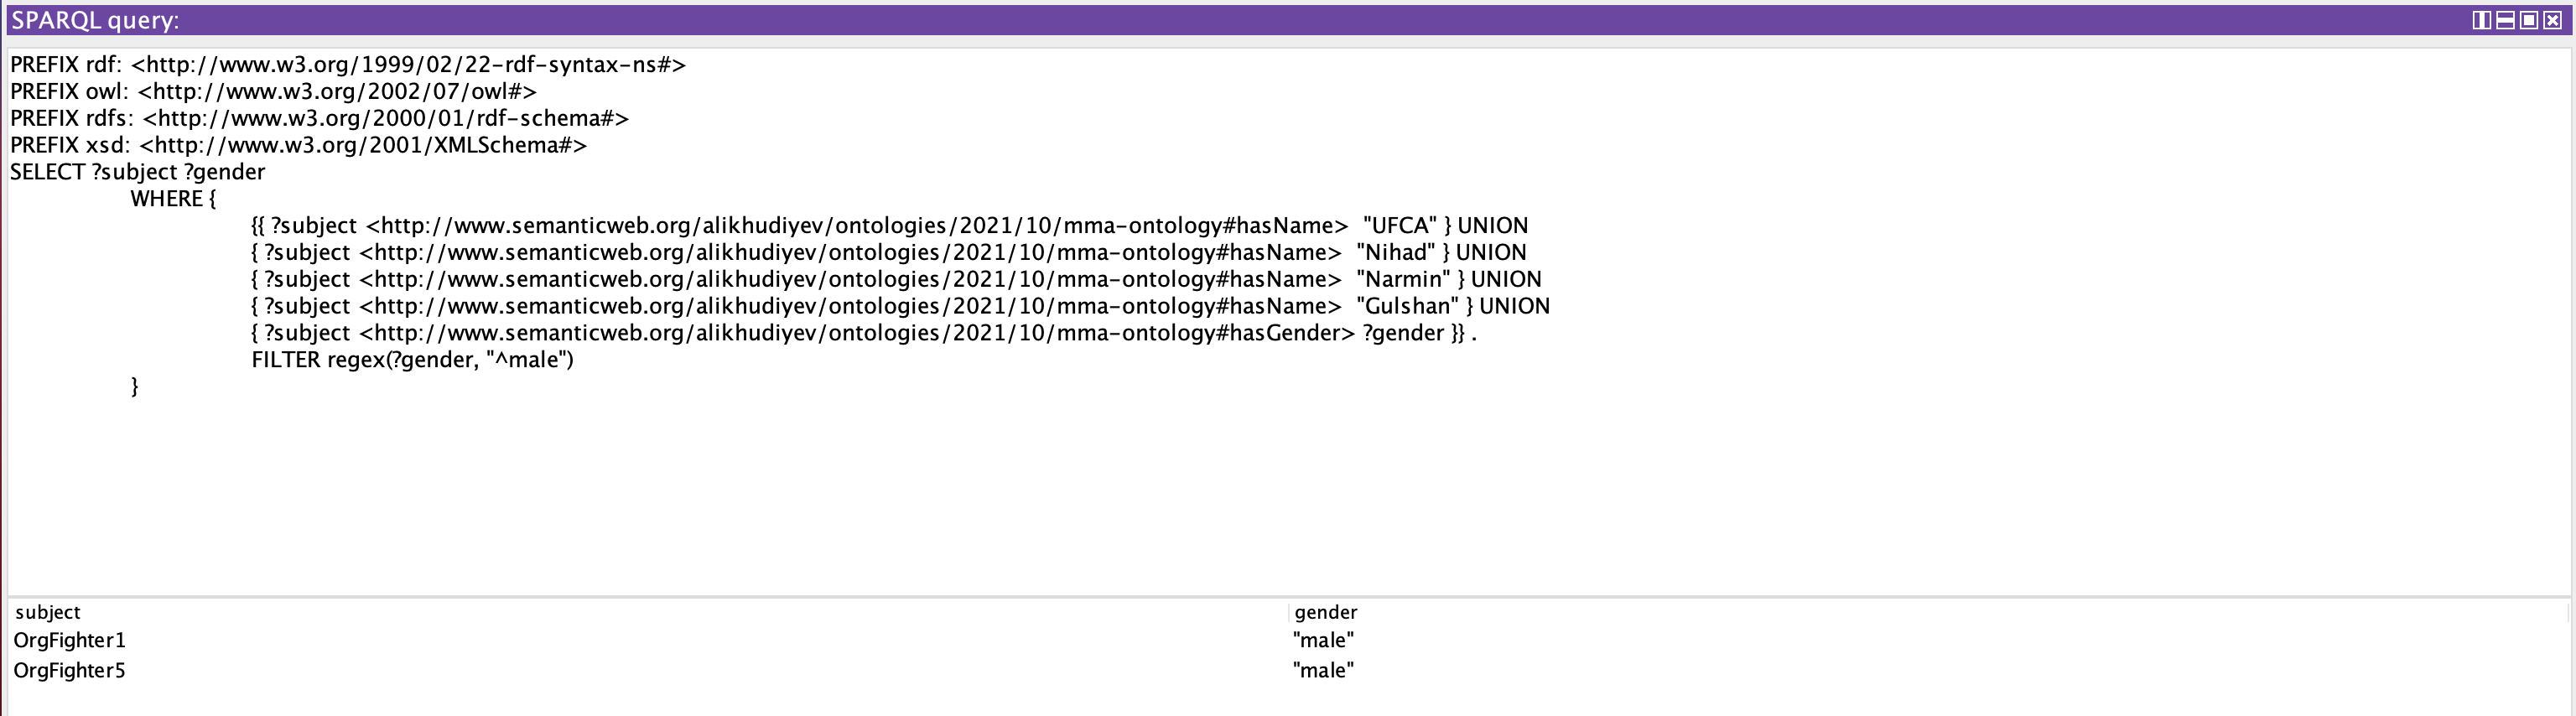
\includegraphics[width=0.8\textwidth]{resources/sparql3.png}
	\caption{Query 2}
	\label{fig:sparql3}
\end{figure}

\section{Reasoning with Pellet}
\subsection{Consistency check}
First thing after the initial development of an ontology is to test it by running the reasoner. There are 2 possibilities after running the reasoner: the ontology is inconsistent or everyhing works 
just fine. The MMA ontology is simply consistent for the matter of well-developed concepts and relations. However, I demonstrate a few cases in which the system would be inconsistent:

\begin{enumerate}
	\item Assigning irreleant weight to a fighter fighting in a certain division (violates \textit{division weight} rule)
	\item Creating a new CEO with a unique name and assigning him/her to the already assigned Organization (violates functional \textit{ownedBy} relation or functional \textit{hasName} relation)
	\item Making a male vs. female fight (violates \textit{same fighter gender} rule)
	\item Making different weight classes to fight (violates \textit{equal fighter weights} rule)
	\item Assigning wrong data type value to an individual through some data property (violates data type restriction)
	\item Giving more than 1 name/birth date/gender to a person (violates max cardinality rule of functional relations)
	\item Making 3 different fighters fight in the same fight (violates max cardinality rule of a fight)
\end{enumerate}

There are many situtations in which the knowledge base would be considered inconsistent, however, underlying principles of consistency are not as many as specific cases. To illustrate some of those 
principles in MMA ontology, I demonstrate examples for \textit{data type violation} and \textit{max cardinality violation} in different cases. The firt 6 cases shown above are illustrated in the 
figure given below.

\begin{figure}[H]
\centering
\begin{subfigure}{.3\textwidth}
	\centering
	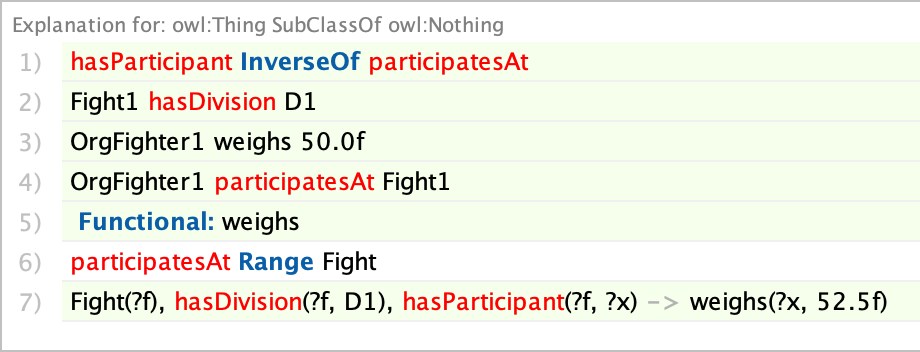
\includegraphics[width=.9\linewidth]{resources/incons1.png}
	\caption{Inconsistency 1}
	\label{fig:sub11}
\end{subfigure}%
\begin{subfigure}{.3\textwidth}
	\centering
	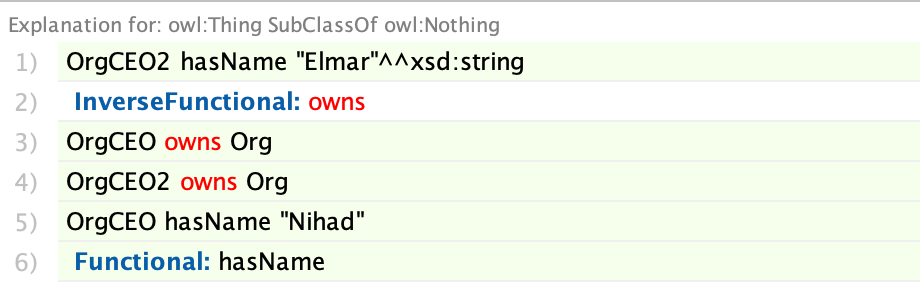
\includegraphics[width=.9\linewidth]{resources/incons2.png}
	\caption{Inconsistency 2}
	\label{fig:sub12}
\end{subfigure}%
\begin{subfigure}{.3\textwidth}
	\centering
	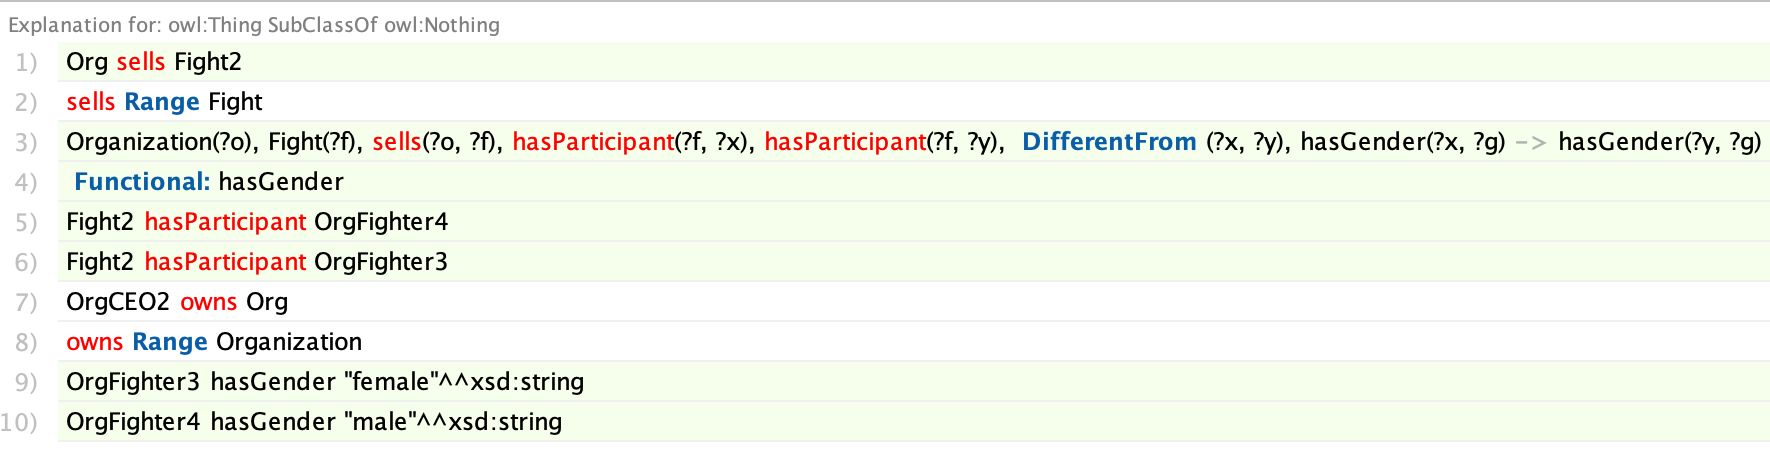
\includegraphics[width=.9\linewidth]{resources/incons3.png}
	\caption{Inconsistency 3}
	\label{fig:sub13}
\end{subfigure}

\begin{subfigure}{.3\textwidth}
	\centering
	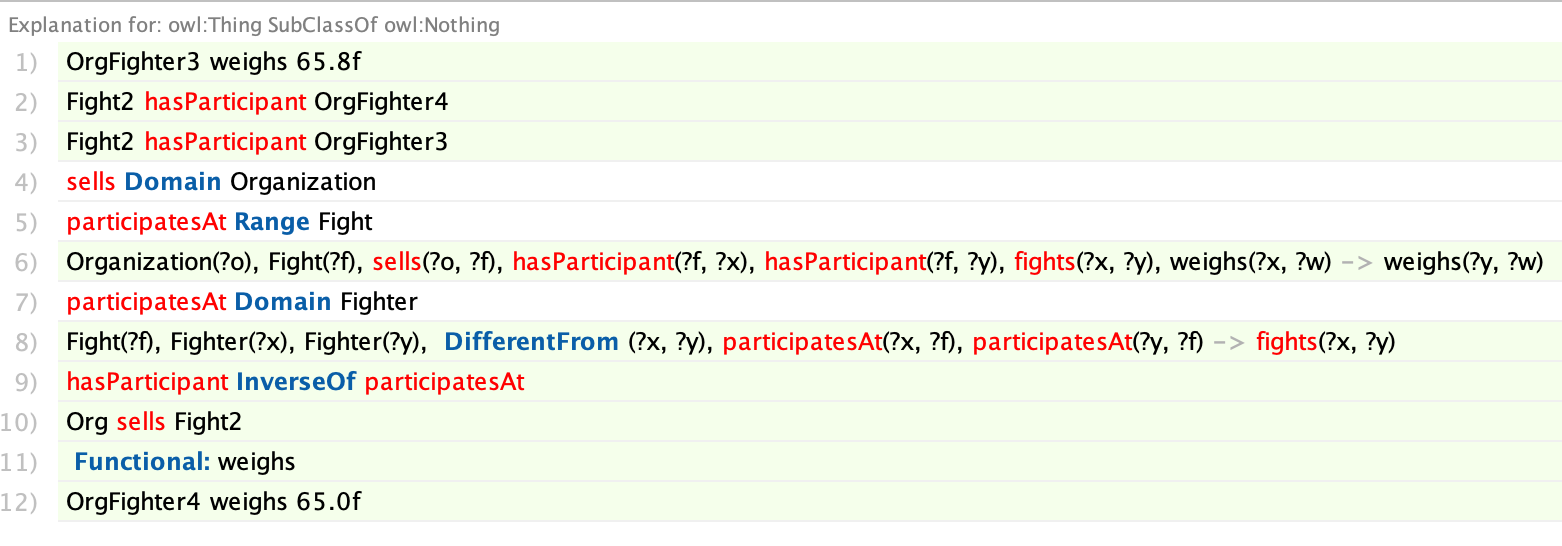
\includegraphics[width=.9\linewidth]{resources/incons4.png}
	\caption{Inconsistency 4}
	\label{fig:sub21}
\end{subfigure}%
\begin{subfigure}{.3\textwidth}
	\centering
	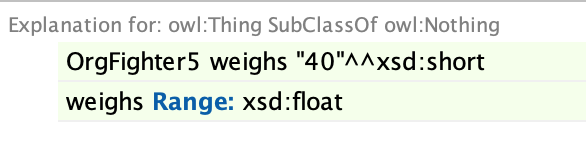
\includegraphics[width=.9\linewidth]{resources/incons5.png}
	\caption{Inconsistency 5}
	\label{fig:sub22}
\end{subfigure}%
\begin{subfigure}{.3\textwidth}
	\centering
	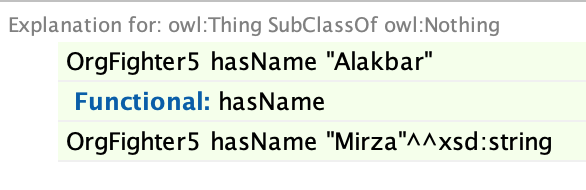
\includegraphics[width=.9\linewidth]{resources/incons6.png}
	\caption{Inconsistency 6}
	\label{fig:sub23}
\end{subfigure}
\caption{Inconsistency explanations given by Prot\'eg\'e}
\label{fig:incons_protege}
\end{figure}

\subsection{Inferences made by Pellet}
\textit{Pellet} is OWL 2 DL reasoner developed in Java that provides functionality for consistency checking of ontologies, computing classification hierarchy, explaining inferences and answering 
to SPARQL queries. \textit{Pellet} can also be used with Jena or OWL-API libraries although none of them are explicitly used in the MMA ontology development. Giving the list of individuals, \textit{Pellet} 
can infer their types, object properties, data properties, relations with other individuals(i.e., \textit{sameAs} or \textit{differentFrom}). The most important and/or interesting inferences for 
individuals are shown in the table below\footnote{For more inferences made by Pellet, see table \ref{tab:all_individuals}(appendix \ref{appendix:individuals}).}.

\begin{table}[H]
	\centering
	\begin{tabular}{|c|c|}
		\hline
		\textbf{Individual} & \textbf{Inferred} \\
		\hline
		Org & occupies LocAz \\
			& ownedBy OrgCEO2, ownedBy OrgCEO \\
			& paysBonus OrgFighter2 \\
		\hline
		OrgCEO & CEO \\
			& sameAs OrgCEO2 \\
		\hline
		OrgCEO2 & CEO \\ 
			& sameAs OrgCEO \\
			& hasName Nihad \\
		\hline
		OrgFighter1 & Fighter \\
			& fights OrgFighter2 \\
			& loses Fight1 \\
			& weighs 52.5 \\
		\hline
		OrgFighter2 & fights OrgFighter1 \\
			& participatesAt Fight1 \\
			& wins Fight1 \\
			& hasGender male, weighs 52.5 \\
		\hline
		Fight1 & Fight \\
			& hasGivenScore FightScore1\_1 \\
			& hasParticipant OrgFighter1 \\
		\hline
	\end{tabular}
	\caption{Individuals}
	\label{tab:inferred}
\end{table}

The individual \textit{OrgCEO} was found to be a CEO by Pellet because of equivalence relation - an individual is CEO if it is a person and it owns an organization. In the other hand, due to subsumption 
the reaoner was able to find that the individuals \textit{OrgCEO}, \textit{OrgFighter1}, \textit{OrgJudge1}, etc. are of type \textit{NamedEntities}. These results concerning subsumption relations can 
be observed by using \textit{DL Query} in Prot\'eg\'e since it does not display this information by default which is probably an interface bug. The reasoner also found out that \textit{OrgCEO} and 
\textit{OrgCEO2} are actually the same instances and the reason is the maximum cardinality of the property called \textit{owns} which is one. Since each individual owned the same organization, it was 
deduced that these individuals are the same and therefore, \textit{OrgCEO2} has also the same name(Nihad) as \textit{OrgCEO}.

\begin{figure}[H]
	\centering
	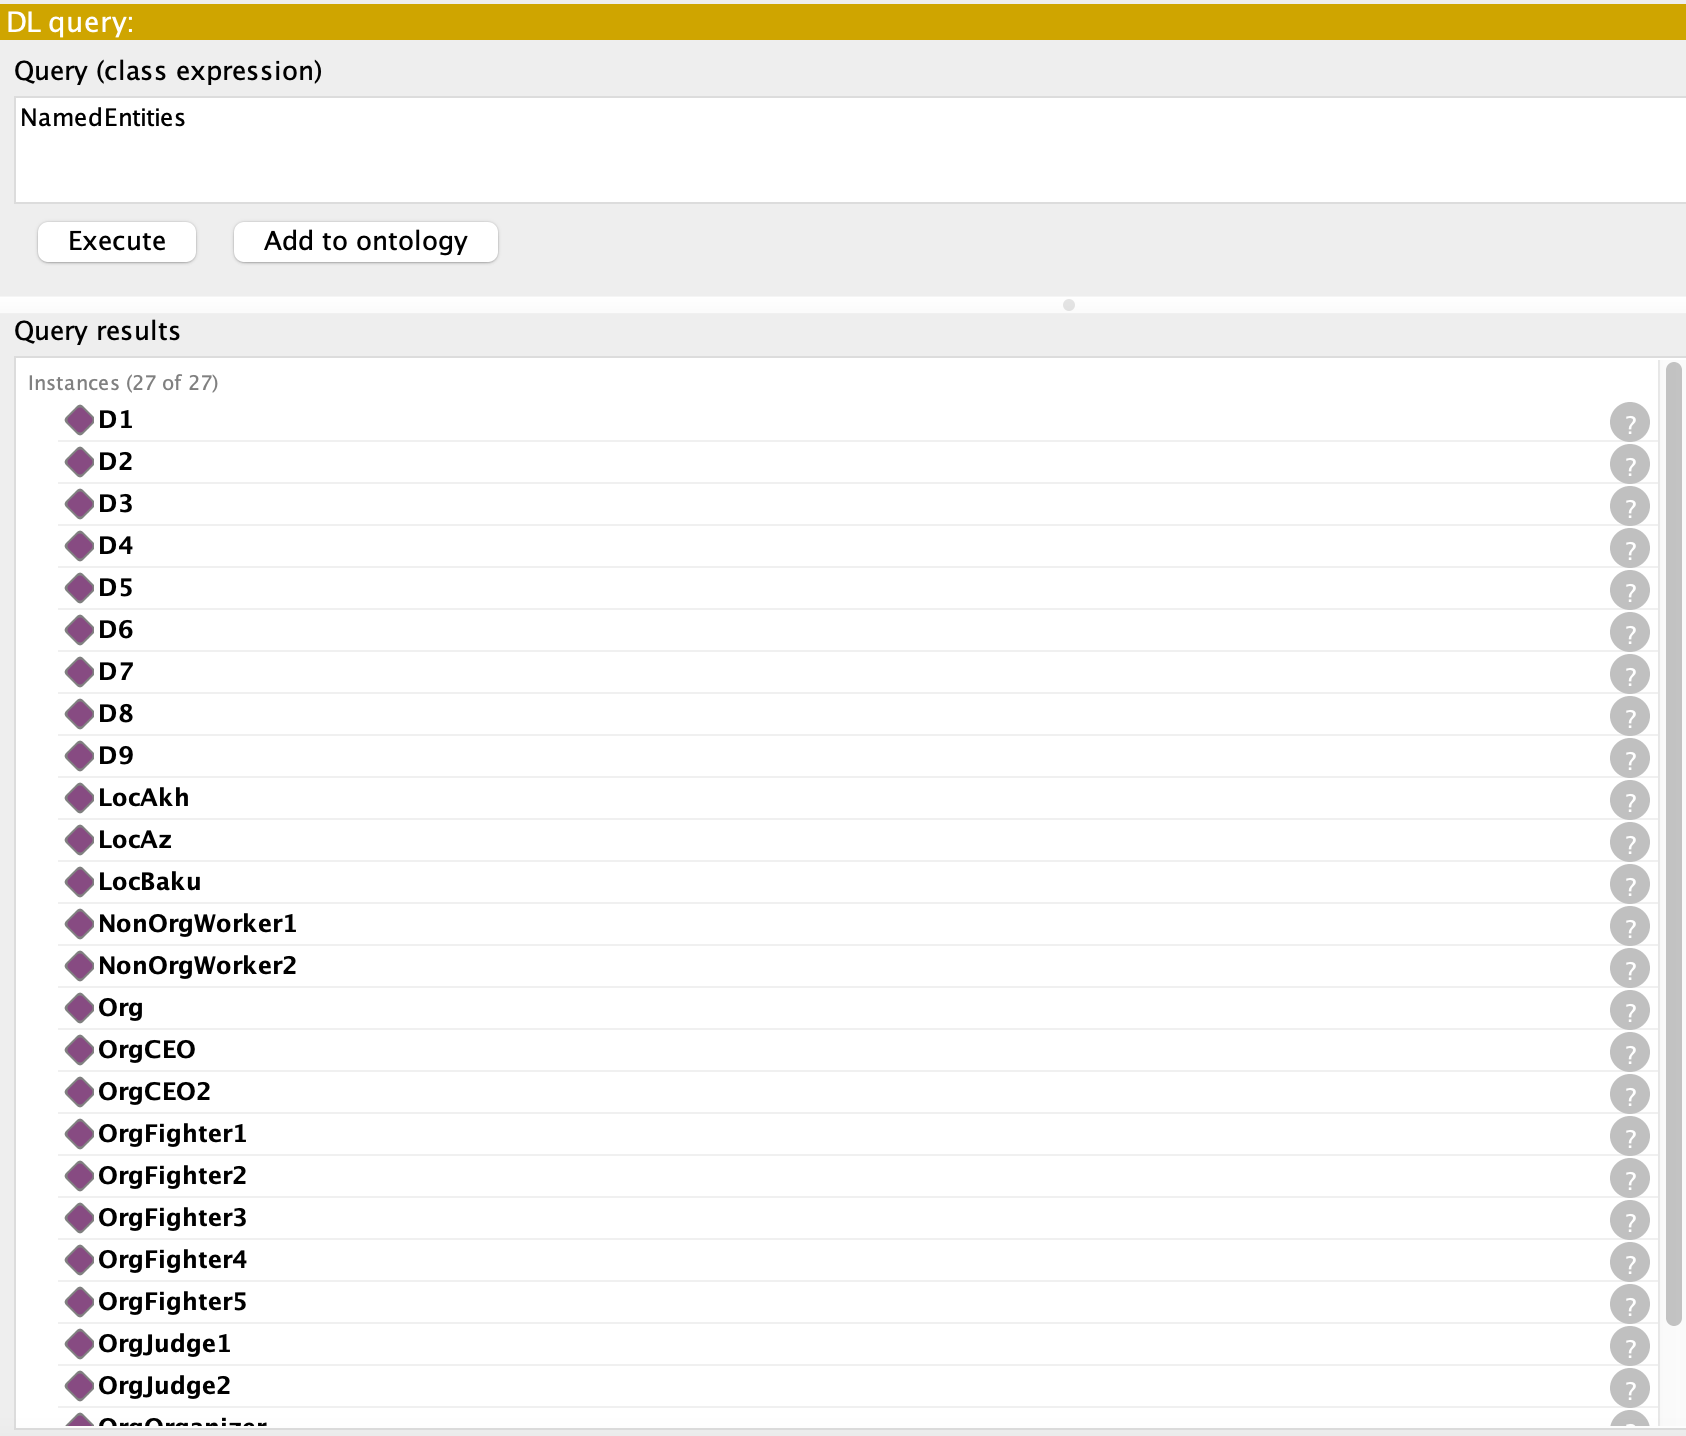
\includegraphics[width=0.7\textwidth]{resources/dl_query.png}
	\caption{DL Query results}
	\label{fig:dl_query}
\end{figure}

Other than using equivalences, subsumptions, disjutions, Pellet is able to infer the types of individuals just by looking at the defined properties on them. For example, the type of \textit{OrgFighter1} 
was found to be Fighter not limited to but simply because of the property \textit{participatesAt} which has a domain initialized as Fighter. Likewise, \textit{OrgCEO} is CEO not only because of class 
equivalence but also because of the given domain of \textit{owns} property.

\subsection{Assumptions used in OWL}
OWL has a couple of assumptions about any ontology: \textit{open world assumption} and \textit{non-unique name assumption}. These assumptions alter the process of inference significantly.
\textit{Open world assumption} states that an unobserved piece of information does not necessarily imply its falsity and \textit{non-unique name assumption} points us to the possbility of two 
different names/representations referring to the same object. Contrary to \textit{closed world assumption}, where unobserved fact is false, and \textit{unique name assumption}, where 
every object has a unique name, these assumptions help us to be more expressive in trade-off with the increased computational cost. 

As most of the ontologies developed in OWL, the MMA ontology has also showcases for OWA(Open World Assumption) and Non-unique Name Assumption. For example, creating an extra tenth individual 
of class \textit{Division} would result with an inconsistency in the knowledge base with CWA(Closed World Assumption) whereas it is totally fine in our case due to OWA and Non-unique Name Assumption.
Since in the definition(see \ref{formula:axiom_division}) of the \textit{Division} class, the individual D10 is not explicitly mentioned, CWA leads to inconsistency. However, it is totally fine with 
OWA since D10 could be the same individual as as any D0-9 which is not restricted by UNA(Unique Name Assumption). In fact, when the reasoner is started in Prot\'eg\'e, it tries to find new 
information about D10 and if not found, it has the ability to say "I don't know" by not giving an inconsistency error and not infering its equivalent individual at the same time. However, if its 
name is given through the predicate \textit{hasName}, it is able to tell whether the knowledge base has inconsistency or D10 is actually the same as some other D0-9 individual. The figures below 
illustrate this process:

\begin{figure}[H]
\centering
\begin{subfigure}{.3\textwidth}
	\centering
	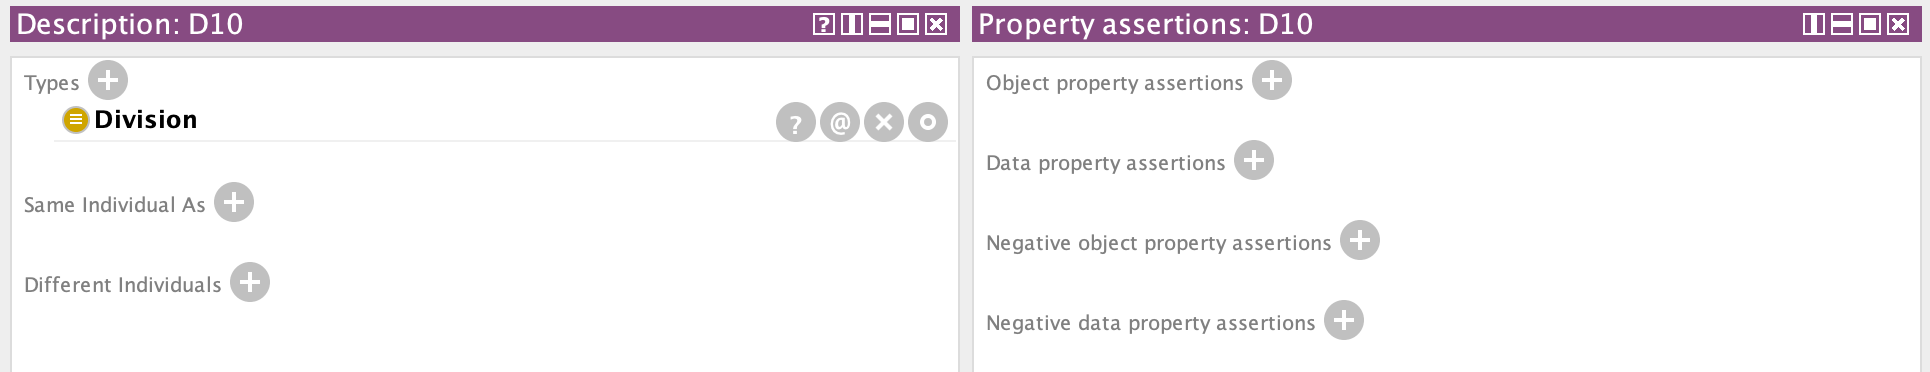
\includegraphics[width=.9\linewidth]{resources/D10_unknown.png}
	\caption{Not enough information \\ to infer anything}
	\label{fig:d10_unknown}
\end{subfigure}%
\begin{subfigure}{.3\textwidth}
	\centering
	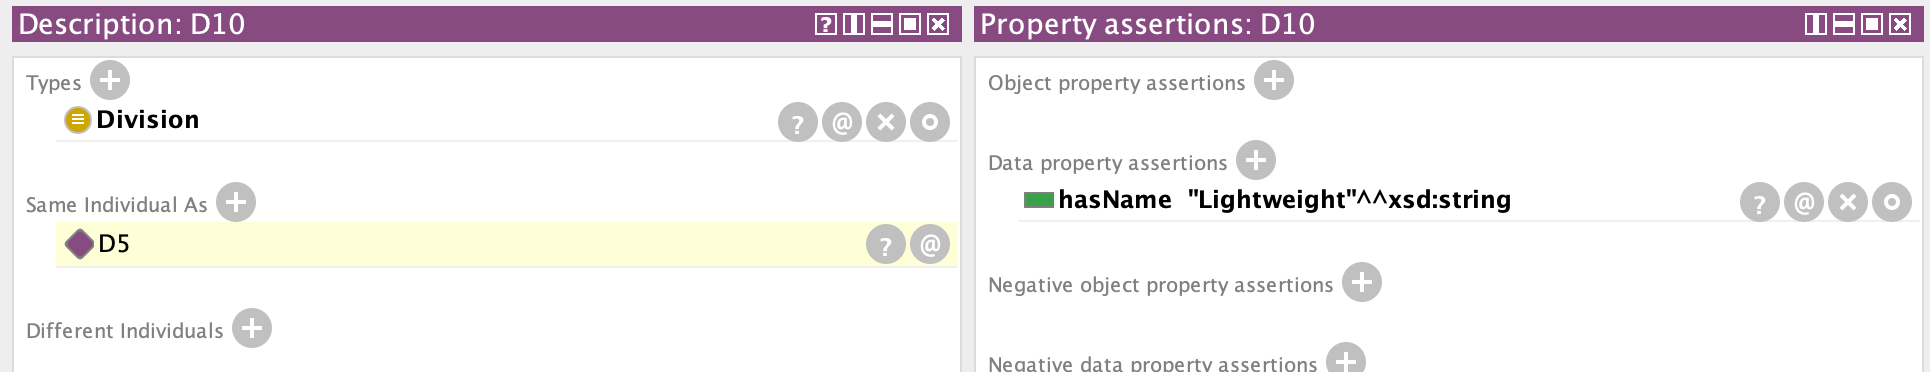
\includegraphics[width=.9\linewidth]{resources/D10_known.png}
	\caption{Enough information to \\ infer the individual the same \\ as with D10 since \textit{hasName} \\ has functional property}
	\label{fig:d10_known}
\end{subfigure}%
\begin{subfigure}{.3\textwidth}
	\centering
	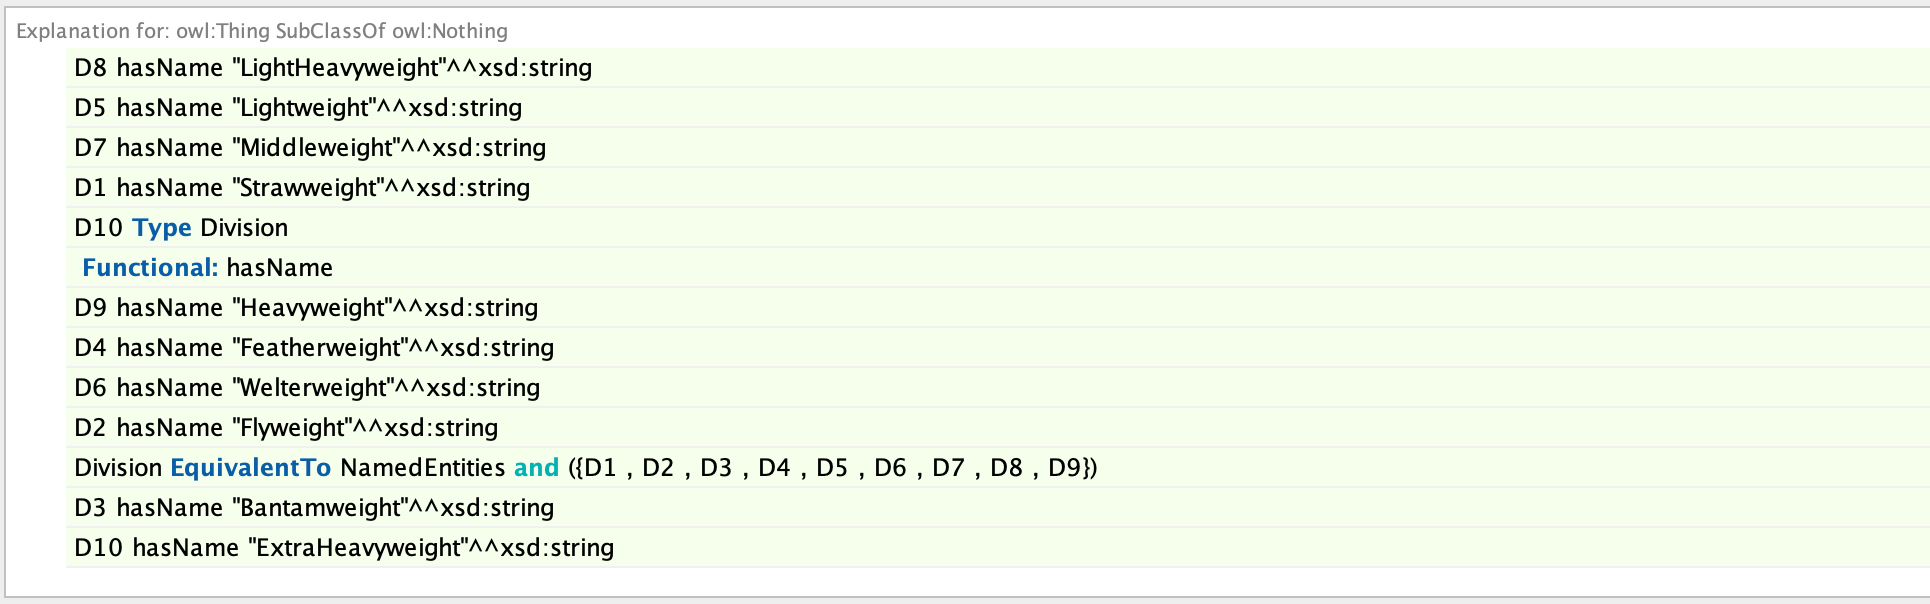
\includegraphics[width=.9\linewidth]{resources/D10_inconsistent.png}
	\caption{Enough information to deduce inconsistency since there have to be 9 individuals in \textit{Division} each of which has to have unique name(\textit{xsd:string}) and there are 10 individuals of \textit{Division} with 10 different names}
	\label{fig:d10_inconsistent}
\end{subfigure}
\caption{OWL Assumptions Showcases}
\label{fig:owl_assumptions_showcases}
\end{figure}

Another showcase for non-unique name assumption would be the use \textit{differentFrom} relation in the relevant rules such as \textit{FightWinnerLoserRule}, \textit{FightDrawerRule} and so on. 
\textit{FightWinnerLoserRule}(see \ref{formula:swrl_winner_loser}) is to detect the loser of the fight based on the winner whereas \textit{FightDrawerRule}(see \ref{formula:swrl_drawers}) is to decide whether 
the fighters finish the fight with a draw based on their post fight scores. If the \textit{differentFrom(?x, ?y)} was not included explicity in \textit{FightWinnerLoserRule}, it would imply that 
any same fighter loses the fight which is won by him/her which is illogical and is prevented by indicating that the participants of the fight have to different from each other. Likewise, if the 
\textit{fights(?x, ?y)} was not included explicitly in \textit{FightDrawerRule}, it would imply that any fighter draws the fight without any affect of his/her score since when $x=y$, both fighter 
seem to have the same score and thus, draws the participated fight. The use of relation \textit{fights(?x, ?y)} is just as good as using \textit{differentFrom(?x, ?y)} since it is irreflexive, 
meaning that it cannot take the same element(fighter) as a domain and range at the same time.

\begin{figure}[H]
\centering
\begin{subfigure}{.5\textwidth}
	\centering
	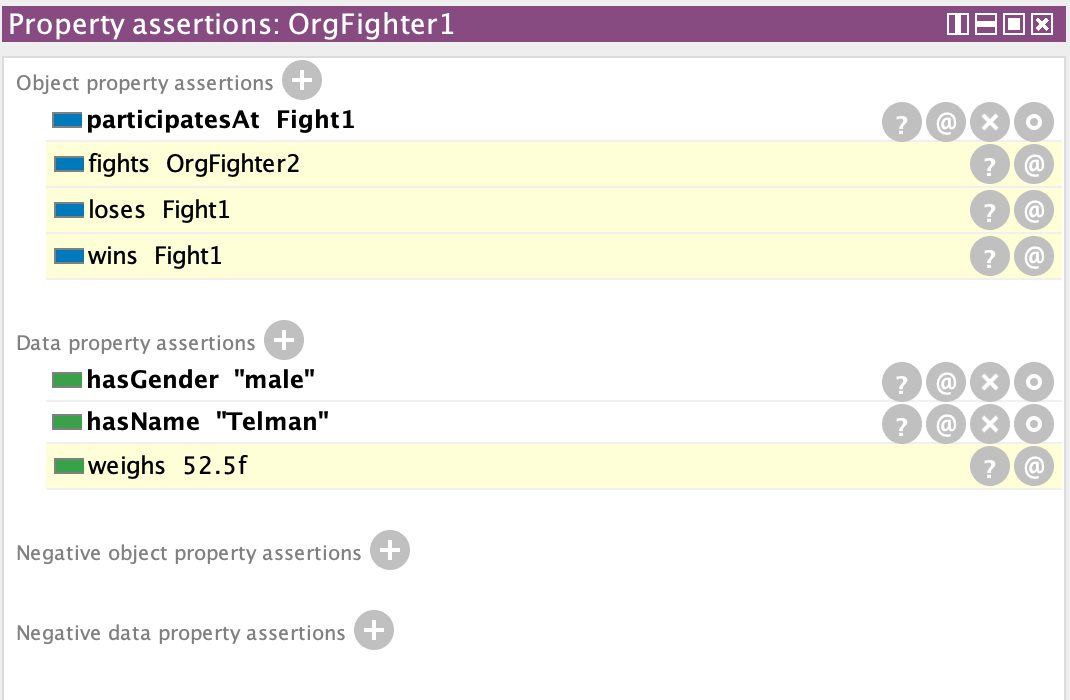
\includegraphics[width=.9\linewidth]{resources/rule_implication_1.png}
	\caption{\textit{FightWinnerLoserRule} without \textit{differentFrom} relation}
	\label{fig:rule_implication_1}
\end{subfigure}%
\begin{subfigure}{.5\textwidth}
	\centering
	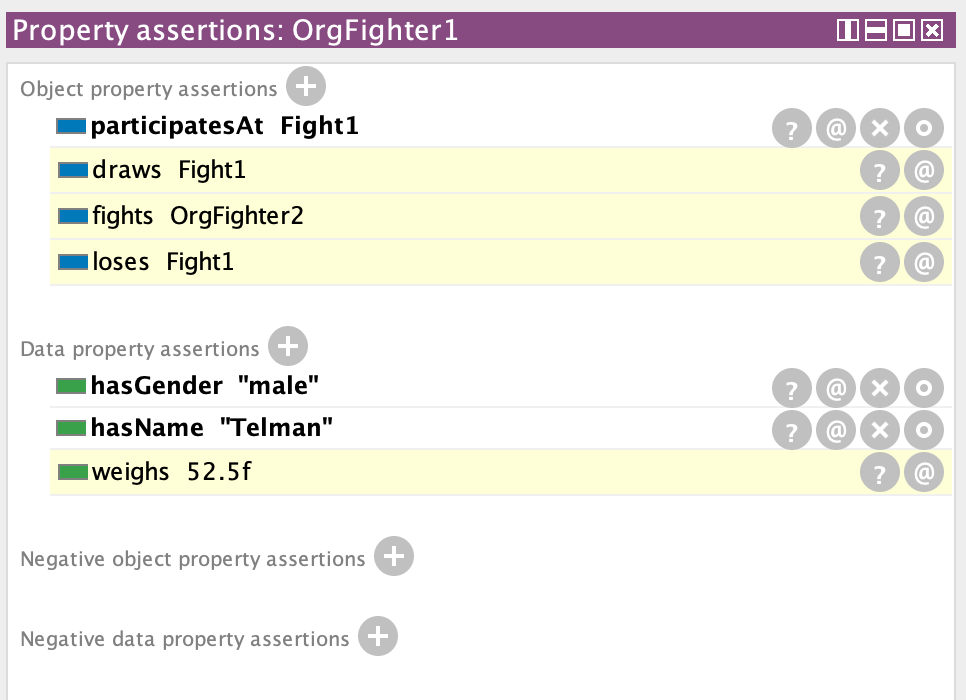
\includegraphics[width=.9\linewidth]{resources/rule_implication_2.png}
	\caption{\textit{FightDrawerRule} without \textit{fights} relation}
	\label{fig:rule_implication_2}
\end{subfigure}
\caption{OWL Assumptions Showcases}
\label{fig:rule_implications}
\end{figure}

\section{Evaluation \& Conclusion}
OWL and SWRL help us to create ontologies with certain subset of first order logic that makes the inference decidable. To do so, it sacrifices some sort of expressiviness that could be otherwise used to 
develop certain ontologies(e.g. an ontology that requires creation of new individuals under some conditions). Another type of problem may arise when trying to represent object states that is dynamic over time 
since there is no concept of time in OWL and SWRL. Consider we want to simulate \textit{Conway's Game of Life}\footnote{\url{https://en.wikipedia.org/wiki/Conway\%27s\_Game\_of\_Life}} by using SWRL rules. 
Since there are cells that are either alive or dead depending on the state of the neighbours, it is not very intuitive to represent a cell which can transform from being dead to alive or vice versa as 
iterations are developed. However, we could still simulate the GoL by representing the concept of time/iteration as an extra dimension. After thinking on the proper way of representing time, I settled in the 
following representation: \textit{each individual cell has its own (current) time or iteration rather than a global notion of time}. This decision comes from the realization that rules can be applied 
randomly when relevant which interrupts the synchronization between cell states and the iteration that they are in. So, rather than having a global notion of iteration, each cell has its own sense of 
iteration which is developed as the reasoner processes or does some transformation upon the cell.

\begin{figure}[H]
	\centering
	\begin{align*}
	\text{Time}&(T) \\
	\text{AliveCell}&(c1) \\
	\text{DeadCell}&(c2) \\
	\text{DeadCell}&(c3) \\
	\text{AliveCell}&(c4) \\
	\text{Time}(T) \land \text{hasValue}(T, t) &\implies \text{hasValue}(T, t+1)
	\end{align*}
	\caption{Notion of global time}
\end{figure}

\begin{figure}[H]
	\centering
	\begin{align*}
	Cell&(c1) \\
	Cell&(c2) \\
	Cell&(c3) \\
	Cell&(c4) \\
	isLiveAt&(c1, 1) \\
	isLiveAt&(c2, -1) \\
	isLiveAt&(c3, -1) \\
	isLiveAt&(c4, 1) \\
	\text{Cell}(c) \land \text{isLiveAt}(c, t) \land \text{hasSufficientNeighbours}&(c, t) \land \text{isNegative}(t) \implies \text{isLiveAt}(c, 1-t) \\
	\text{Cell}(c) \land \text{isLiveAt}(c, t) \land \text{hasSufficientNeighbours}&(c, t) \land \text{isPositive}(t) \implies \text{isLiveAt}(c, 1+t) \\
	\text{Cell}(c) \land \text{isLiveAt}(c, t) \land \text{hasInsufficientNeighbours}&(c, t) \land \text{isNegative}(t) \implies \text{isLiveAt}(c, -1+t) \\
	\text{Cell}(c) \land \text{isLiveAt}(c, t) \land \text{hasInsufficientNeighbours}&(c, t) \land \text{isPositive}(t) \implies \text{isLiveAt}(c, -1-t) \\
	\text{Cell}(c) \land \text{hasNeighbour}(c, c1) \land \text{isLiveAt}(c1, t) \land \dots \land &\text{ isPositive}(t) \implies \text{hasSufficientNeighbours}(c, t) \\
	\text{Cell}(c) \land \text{hasNeighbour}(c, c1) \land \text{isLiveAt}(c1, t) \land \dots \land &\text{ isPositive}(t) \implies \text{hasInsufficientNeighbours}(c, t)
	\end{align*}
	\caption{Notion of local time}
\end{figure}

The predicate \lstinline{isLiveAt(cell, t)} represents an alive cell when $t>0$ and a dead cell when $t<0$. The analogy here is that time is bidirectional; positive time represents the time in our world 
and negative time represents the time in afterlife. So, \lstinline{isLiveAt(cell, 3)} indicates that the cell is alive at the iteration 3 and \lstinline{isLiveAt(cell, -4)} means that the cell is alive 
at the iteration 4 in afterlife, in other words, the cell is dead at iteration 4 (in our world). A cell is alive in our world when it is dead in the afterlife and vice versa. This representation avoids 
the creation of new cells (as it is also prohibited in DL) and helps us to illustrate the notion of iteration/time. However, the above shown rules are not the only ones required to build such interesting 
ontology and the missing pieces that I have not intentionally mentioned is the formulas describing \lstinline{hasSufficientNeighbours}(cell, t) and \lstinline{hasInsufficientNeighbours}(cell, t); these 
are also updates through the process. In fact, \lstinline{hasSufficientNeighbours(cell, t)} is updated to indicate that if cell has sufficient number of neighbours at iteration $t$ to keep living 
(if live before) or turn to an alive cell (if dead before) at the consequent($t+1$) iteration. It is the opposite case for \lstinline{hasInsufficientNeighbours(cell, t)} which is updated to indicate 
whether a cell has less or more than enough live neighbours at the iteration $t$.

Working on this project made me realize some facts about \textit{difficulty of developing a good ontology}, \textit{computation complexity of logic}, \textit{integration of time to ontologies} and finally 
\textit{bugs of Prot\'eg\'e software}. Developing a good ontology is not as easy as it may seem at the first glance, concepts and relations between them have to be carefully observed before discussing 
implementation details. While observing the true nature of a given problem, we have to also think about the assumptions that we make because our predictions lies behind our assumptions. Although DL is 
a decidable subset of FoL(First Order Logic), it is not as expressive which is an obvious trade-off. Finally, I gave Prot\'eg\'e a try to develop this particular project and encountered several problems 
along the way. I believe, there is a potential to develop the software and reduce the bugs.

\newpage
\section*{Appendix}
\begin{appendix}
	\section{Properties}
	\label{appendix:object_props}
	\begin{table}[H]
		\centering
		\begin{tabular}{|m{0.15\textwidth}|m{0.17\textwidth}|m{0.17\textwidth}|m{0.17\textwidth}|m{0.2\textwidth}|}
			\hline
			\textbf{Relation} & \textbf{Domain} & \textbf{Range} & \textbf{Type} & \textbf{Description} \\
			\hline
			hasDivision & Fight & Division & functional & A fight has only one division \\
			\hline
			buys & NonOrgWorker & Fight & - & Any non organization worker can buy a fight \\
			\hline
			draws & Fighter & Fighter & regular & Fighters can draw \\
			\hline
			fights & Fighter & Fighter & symmetric, irreflexive & A fighter fights against another fighter \\
			\hline
			gives & Judge & FightScore & - & Judge gives the final score(s) \\
			\hline
			hasParticipant & Fight & Fighter & inverse (participatesAt) & Fight has a participating fighter \\
			\hline
			sells & Organization & Fight & regular & Organization sells fights \\
			\hline
			hasScore & Fight & FightScore & inverse (refersTo), inverse functional & Fight has a final score \\
			\hline
			isFor & FightScore & Fighter & functional & Fight score is given to a particular fighter \\
			\hline
			loses & Fighter & Fighter & inverse (wins) & Fighter can lose to another fighter \\
			\hline
			occupies & PhysicalEntities & Location & transitive & Physical entity occupies(located at) some location \\
			\hline
			organizes & Organizer & Fight & - & Organizer(s) organize(s) fight(s) \\
			\hline
			ownedBy & Organization & CEO & inverse (owns), functional & Organization is owned by a single CEO \\
			\hline
			owns & CEO & Organization & inverse (ownedBy), inverse functional & Organization is owned by a single CEO \\
			\hline
			participatesAt & Fighter & Fight & inverse (hasParticipant) & Fighter participates at a fight by fighting \\
			\hline
			pays & Organization & OrgWorker & inverse (worksAt) & Organization pays salary to the organization workers \\
			\hline
			refersTo & FightScore & Fight & inverse (hasScore), functional & Every fight score is given to a particular fight \\
			\hline
			sells & Organization & Fight & inverse functional & Organization sells fight(s) \\
			\hline
			wins & Fighter & Fight & - & Fighter can win a fight \\
			\hline
			worksAt & OrgWorker & Organization & inverse (pays) & Organization worker works at an organization \\
			\hline
		\end{tabular}
		\caption{Object properties}
		\label{tab:object_props}
	\end{table}

	\section{Individuals}
	\label{appendix:individuals}
	\begin{table}[H]
		\centering
		\begin{tabular}{|c|c|c|}
			\hline
			\textbf{Individual} & \textbf{Asserted} & \textbf{Inferred} \\
			\hline
			Org & Organization & occupies LocAz \\
				& sells Fight1 & ownedBy OrgCEO2 \\
				& sells Fight2 & ownedBy OrgCEO \\
				& occupies LocBaku & paysBonus OrgFighter2 \\
				& hasName UFCA & \\
			\hline
			OrgCEO & Person & CEO \\
				& owns Org & sameAs OrgCEO2 \\
				& hasName Nihad & \\
			\hline
			OrgCEO2 & owns Org & CEO \\
				& & sameAs OrgCEO \\
				& & hasName Nihad \\
			\hline
			OrgFighter1 & participatesAt Fight1 & Fighter \\
				& hasGender male & fights OrgFighter2 \\
				& hasName Telman & loses Fight1 \\
				& & weighs 52.5 \\
			\hline
			OrgFighter2 & Fighter & fights OrgFighter1 \\
				& hasName Bashir & participatesAt Fight1 \\
				& & wins Fight1 \\
				& & hasGender male \\
				& & weighs 52.5 \\
			\hline
			OrgFighter3 & Fighter & draws Fight2 \\
				& hasName Daniz & fights OrgFighter4 \\
				& weighs 65.8 & participatesAt Fight2 \\
				& hasGender female & \\
				& warBorn 1990-01-01T00:00:00 & \\
			\hline
			OrgFighter4 & Fighter & draws Fight2 \\
				& hasName Narmin & fight OrgFighter3 \\
				& & participatesAt Fight2 \\
				& & hasGender female \\
				& & weighs 65.8 \\
			\hline
			Fight1 & hasDivision D1 & Fight \\
				& hasGivenScore FightScore1\_2 & hasGivenScore FightResult1\_1 \\
				& hasParticipant OrgFighter2 & hasParticipant OrgFighter1 \\
				& costs 25.0 & \\
			\hline
			Fight2 & Fight & \\
				& hasGivenScore FightScore2\_1 & \\
				& hasGivenScore FightScore2\_2 & \\
				& hasParticipant OrgFighter3 & \\
				& hasParticipant OrgFighter4 & \\
				& costs 18.0 & \\
			\hline
			FightScore1\_1 & FightScore & \\
				& isFor OrgFighter1 & \\
				& refersTo Fight1 & \\
				& hasScore 15 & \\
			\hline
			FightScore1\_2 & FighScore & refersTo Fight1 \\
				& isFor OrgFighter2 & \\
				& hasScore 17 & \\
			\hline
			FightScore2\_1 & FighScore & refersTo Fight2 \\
				& isFor OrgFighter 3 & \\
				& hasScore 10 & \\
			\hline
			FightScore2\_2 & FighScore & refersTo Fight2 \\
				& isFor OrgFighter4 & \\
				& hasScore 10 & \\
			\hline
			% LocAz & Location & \\
			% 	& hasName Azerbaijan & \\
			% \hline
			LocBaku & occupies LocAz & Location \\
				& hasName Baku & \\
			% \hline
			% LocAkh & Location & occupies LocAz \\
			% 	& occupies LocBaku & \\
			% 	& hasName Akhmadli & \\
			\hline
		\end{tabular}
		\caption{Individuals}
		\label{tab:all_individuals}
	\end{table}

	\section{Graph by Ontograf}
	\label{appendix:ontograf_graph}
	\begin{figure}[H]
		\centering
		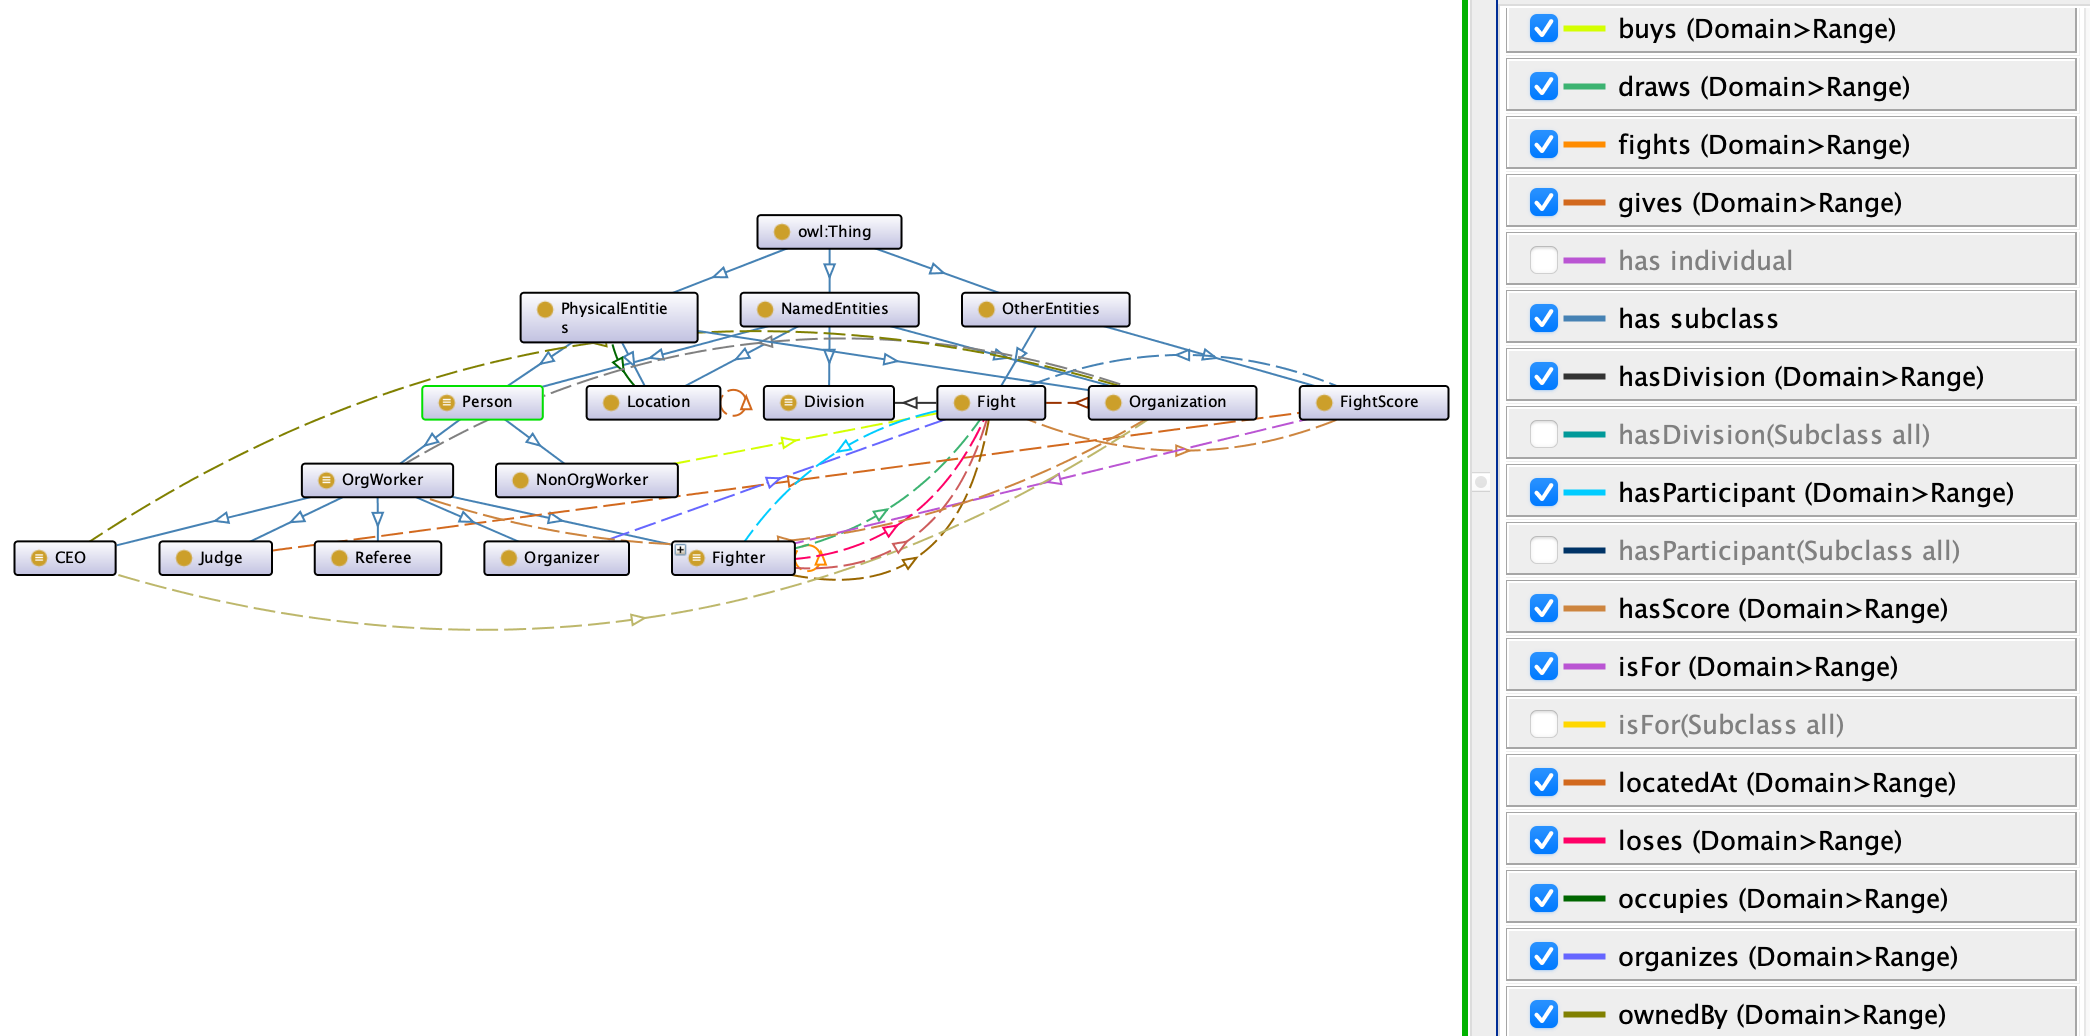
\includegraphics[width=0.8\textwidth]{resources/ontograf.png}
		\caption{Complete graph with arc labels}
		\label{fig:ontograf}
	\end{figure}
\end{appendix}

\end{document}
